%!TeX program = xelatex
\documentclass{SYSUReport}

\setlength{\headheight}{14.5pt}

% 根据个人情况修改
\headl{模式识别大作业}
\headc{基于OULAD数据集的学业风险预警模型研究}
\headr{22320021-陈安康}
\lessonTitle{模式识别课程大作业}
\reportTitle{基于多种机器学习模型的学业风险预警系统设计与实现}
\stuname{陈安康}
\stuid{22320021}
\inst{计算机学院}
\major{计算机科学与技术}
\date{\today}
\usepackage{graphicx}
\usepackage{subcaption}
\begin{document}

% =============================================
% Part 1: 封面
% =============================================
\cover
\thispagestyle{empty} % 首页不显示页码
\clearpage

% =============================================
% Part 2： 摘要
% =============================================
\begin{abstract}
随着在线教育的普及，如何利用海量学习行为数据，提前识别并干预有潜在学业困难的学生，已成为教育数据挖掘领域的重要课题。本项目旨在基于OULAD (Open University Learning Analytics Dataset) 数据集，设计并实现一个模块化的学业风险预警系统，并对多种机器学习模型的性能进行综合评估。

本项目首先构建了一个健壮的数据处理流水线，包括ETL、数据清洗、特征工程和探索性数据分析(EDA)。在此基础上，我们实现并对比了七种主流的机器学习模型，涵盖监督学习（逻辑回归、决策树、随机森林、支持向量机）和无监督学习（K-Means、高斯混合模型EM）。为了追求模型的最优性能，我们引入了Optuna框架进行自动化超参数优化，并利用SHAP (SHapley Additive exPlanations)框架对模型进行深度可解释性分析。

本项目不仅实现了一个端到端的学业风险预测系统，还从准确性、效率、可解释性、复杂度等多个维度，建立了一套完整、公正的模型评估与比较框架。研究成果可为在线教育平台实施个性化干预、提升教学质量提供数据驱动的决策支持。

\textbf{关键字}：学业风险预警；机器学习；OULAD；模型对比；Optuna；SHAP
\end{abstract}
\thispagestyle{empty} % 摘要页不显示页码
\clearpage


% =============================================
% Part 3： 目录页
% =============================================
% 重置页码，并使用罗马数字
\pagenumbering{Roman}
\setcounter{page}{1}
\tableofcontents
\clearpage

% =============================================
% Part 4： 正文内容
% =============================================
% 重置页码，并使用阿拉伯数字
\pagenumbering{arabic}
\setcounter{page}{1}

\section{绪论}
\subsection{研究背景与意义}
随着信息技术的飞速发展，在线学习已成为现代教育的重要组成部分。大规模在线开放课程（MOOCs）等平台积累了海量的学生学习行为数据，这些数据为我们理解学习过程、优化教学策略提供了前所未有的机遇。然而，在线学习环境的开放性和灵活性也带来了新的挑战，如学生学习投入度不高、容易迷失方向、辍学率高等问题。因此，如何利用学习分析技术，主动、准确地识别出有潜在学业困难（at-risk）的学生，并及时给予个性化指导和干预，对于提升在线教育质量、促进教育公平具有至关重要的现实意义。

学业风险预警旨在通过分析学生的历史和实时数据，构建预测模型，判断其未来可能遇到的学习困难或失败风险。一个有效的预警系统能够帮助教学管理者和教师从“事后补救”转变为“事前预防”，将有限的教育资源精准地投入到最需要的学生身上，从而实现个性化教育和精细化管理。

\subsection{OULAD数据集介绍}
本项目采用业界知名的开放大学学习分析数据集（OULAD）\cite{kuzilek2017open}。该数据集包含了英国开放大学（Open University）在2013年和2014年提供的7个模块（课程）的数据。数据是匿名的，包含了学生的人口统计学信息、课程注册信息、学习行为数据（虚拟学习环境VLE中的点击流数据）、以及最终的学业成绩。OULAD数据集的丰富性和完整性使其成为研究学生学习行为和预测学业成果的理想选择。

\subsection{研究内容与目标}
本项目的主要目标是设计并实现一个端到端的学业风险预警系统，并对不同机器学习算法在该任务上的表现进行系统性的对比分析。具体研究内容包括：
\begin{itemize}
    \item \textbf{模块化数据处理流水线构建：} 设计并实现一套从数据提取、转换、加载（ETL）到数据清洗、特征工程和探索性数据分析（EDA）的完整流程。
    \item \textbf{多种机器学习模型实现：} 基于统一的框架，实现并训练七种经典的监督与无监督学习模型，全面覆盖不同算法范式。
    \item \textbf{自动化超参数调优：} 引入Optuna框架，对各模型进行高效的超参数搜索，以发掘其最佳性能。
    \item \textbf{多维度模型性能评估：} 从准确性（Accuracy, Precision, Recall, F1-Score, AUC）、效率（训练时间、预测时间、模型大小）和可解释性（SHAP分析）等多个角度，对模型进行综合评估和比较。
    \item \textbf{研究结论与系统总结：} 总结不同模型的优劣势和适用场景，为解决实际学业预警问题提供决策依据。
\end{itemize}

\section{问题定义}
通过eda数据分析，我发现大多数的学生只有一门课程记录（约为74.48\%）。于此同时，从现实方面出发，研究学生在某一门课程上的表现情况是评估一名学生学业情况的基础。
对于评估标准的制定，课程的最终成绩评定结果是最直接的依据。因此，我们利用OULAD数据集中学生的最终成绩（final\_result），将结果为“Fail”或“Withdrawn”的学生标记为高风险（at\_risk = 1），将结果为“Pass”或“Distinction”的学生标记为低风险（at\_risk = 0）。
因此，本研究将“识别学业困难学生”这一开放性问题，转化为一个明确的、可操作的监督学习分类任务。系统的核心目标即是，仅利用学生在课程前期的学习行为数据，准确地预测其在课程结束时是否会属于at\_risk类别。

\section{模型原理与相关技术}
本章将详细介绍项目中使用的核心机器学习模型及相关支撑技术的原理。

\subsection{监督学习模型}
监督学习模型通过学习带有标签的训练数据（即特征和对应的已知结果），来预测新数据的标签。

\subsubsection{逻辑回归 (Logistic Regression)}
逻辑回归是一种经典的线性分类模型，虽然名为“回归”，但其主要用于解决二分类问题。其核心思想是利用Sigmoid函数将线性回归的连续预测值映射到(0, 1)区间，从而得到一个表示样本属于某个类别的概率。
\begin{equation}
    h_\theta(x) = g(\theta^T x) = \frac{1}{1 + e^{-\theta^T x}}
\end{equation}
其中，$g(z)$是Sigmoid函数。模型通过最大化对数似然函数来学习参数$\theta$，通常使用梯度下降等优化算法求解。逻辑回归模型简单、高效、易于解释（特征的系数直接反映其对结果的影响），是处理分类问题的常用基准模型。

\subsubsection{决策树 (Decision Tree)}
决策树是一种基于树状结构进行决策的非参数学习模型。它通过一系列if-then-else的决策规则，对数据进行递归划分，最终将数据点分配到叶节点的类别中。构建决策树的关键在于如何选择最优的划分特征。常用的划分准则有信息增益（ID3算法）、信息增益率（C4.5算法）和基尼不纯度（CART算法）。
\begin{equation}
    \text{Gini}(D) = 1 - \sum_{k=1}^{K} p_k^2
\end{equation}
决策树模型具有极强的可解释性，其决策过程直观易懂。但单个决策树容易过拟合，对数据中的微小变化敏感。

\subsubsection{随机森林 (Random Forest)}
随机森林是一种基于Bagging思想的集成学习模型，它通过构建并结合多个决策树来进行预测。为了保证基学习器（决策树）之间的差异性，随机森林引入了两种“随机性”：
\begin{itemize}
    \item \textbf{样本随机：} 通过自助采样法（Bootstrap Sampling），为每棵树生成不同的训练子集。
    \item \textbf{特征随机：} 在每个节点进行划分时，不是从所有特征中选择最优特征，而是从一个随机选择的特征子集中进行选择。
\end{itemize}
最终的预测结果由所有决策树投票决定（分类问题）或取平均值（回归问题）。随机森林能够有效克服单决策树的过拟合问题，具有很高的预测精度和鲁棒性，并且能够评估特征的重要性。

\subsubsection{支持向量机 (SVM)}
支持向量机是一种强大的二分类模型，其核心思想是在特征空间中寻找一个能将不同类别样本最大程度分开的最优超平面。这个“最大间隔”是通过求解一个凸二次规划问题得到的。对于线性不可分的数据，SVM通过引入核函数（Kernel Trick），如多项式核、高斯核（RBF），将数据映射到更高维的特征空间，使其在该空间中线性可分。
\begin{equation}
    \min_{\mathbf{w}, b} \frac{1}{2}\|\mathbf{w}\|^{2} \quad \text { s.t. } y_{i}\left(\mathbf{w} \cdot \mathbf{x}_{i}-b\right) \geq 1, i=1, \ldots, n
\end{equation}
SVM特别适用于高维数据和中小样本量问题，并且具有很好的泛化能力。

\subsection{无监督学习模型}
无监督学习模型直接对未标记的数据进行学习，试图发现数据中潜在的结构或模式。

\subsubsection{K-Means聚类}
K-Means是一种经典的划分式聚类算法。其目标是将数据集划分为$K$个簇，使得每个数据点都属于离它最近的簇中心（质心）所代表的簇。算法通过迭代的方式进行，包含两个步骤：
\begin{enumerate}
    \item \textbf{分配步骤：} 将每个数据点分配到其最近的质心所在的簇。
    \item \textbf{更新步骤：} 重新计算每个簇的质心（该簇所有数据点的均值）。
\end{enumerate}
该过程不断重复，直到质心不再发生变化或达到最大迭代次数。K-Means算法简单、高效，但对初始质心的选择和噪声敏感，且假定簇是球形的。

\subsubsection{高斯混合模型 (GMM) 与EM算法}
高斯混合模型（GMM）是一种基于概率模型的聚类方法。它假设数据是由$K$个不同的高斯分布（正态分布）混合生成的。每个高斯分布代表一个簇。GMM比K-Means更灵活，因为它可以适应椭圆形的簇，并且可以为每个数据点提供其属于各个簇的概率。
\begin{equation}
    p(\mathbf{x}) = \sum_{k=1}^{K} \pi_k \mathcal{N}(\mathbf{x} | \boldsymbol{\mu}_k, \boldsymbol{\Sigma}_k)
\end{equation}
GMM的参数（混合系数$\pi_k$，均值$\boldsymbol{\mu}_k$，协方差$\boldsymbol{\Sigma}_k$）通常通过期望最大化（Expectation-Maximization, EM）算法来学习。EM算法是一种迭代优化算法，用于在数据不完整（存在隐变量）的情况下求解参数的最大似然估计。它主要包含以下两个步骤，并交替进行直至收敛：
\begin{enumerate}
    \item \textbf{E步（Expectation）：} 基于当前的参数估计，计算每个数据点 $\mathbf{x}_i$ 由第 $k$ 个高斯分布生成的后验概率（也称为“响应度”）。这个值可以理解为样本 $i$ 属于簇 $k$ 的“软”归属程度。
    \begin{equation}
        \gamma(z_{ik}) = p(z_{ik}=1 | \mathbf{x}_i, \boldsymbol{\theta}) = \frac{\pi_k \mathcal{N}(\mathbf{x}_i | \boldsymbol{\mu}_k, \boldsymbol{\Sigma}_k)}{\sum_{j=1}^{K} \pi_j \mathcal{N}(\mathbf{x}_i | \boldsymbol{\mu}_j, \boldsymbol{\Sigma}_j)}
    \end{equation}
    \item \textbf{M步（Maximization）：} 基于E步计算出的响应度，更新模型参数，以最大化对数似然函数的期望。具体来说，是使用加权的样本来重新计算每个高斯分布的均值、协方差和混合系数。
    \begin{align}
        \boldsymbol{\mu}_k^{\text{new}} &= \frac{\sum_{i=1}^{N} \gamma(z_{ik}) \mathbf{x}_i}{\sum_{i=1}^{N} \gamma(z_{ik})} \\
        \boldsymbol{\Sigma}_k^{\text{new}} &= \frac{\sum_{i=1}^{N} \gamma(z_{ik}) (\mathbf{x}_i - \boldsymbol{\mu}_k^{\text{new}})(\mathbf{x}_i - \boldsymbol{\mu}_k^{\text{new}})^T}{\sum_{i=1}^{N} \gamma(z_{ik})} \\
        \pi_k^{\text{new}} &= \frac{\sum_{i=1}^{N} \gamma(z_{ik})}{N}
    \end{align}
\end{enumerate}


\subsection{关键支撑技术}
\subsubsection{Optuna超参数优化}
超参数的选择对机器学习模型的性能至关重要。手动调参耗时耗力且效率低下。Optuna是一个专为机器学习设计的自动化超参数优化框架 \cite{akiba2019optuna}。它采用先进的采样和剪枝算法（如TPE），能够智能地在巨大的参数空间中进行搜索，比传统的网格搜索和随机搜索更高效。在本项目中，我们利用Optuna为每个模型自动寻找最佳的超参数组合。

\subsubsection{SHAP可解释性分析}
虽然一些复杂模型（如随机森林）性能强大，但其“黑箱”特性使其决策过程难以理解。SHAP (SHapley Additive exPlanations) 是一种基于博弈论的先进模型解释框架 \cite{lundberg2017unified}。它通过计算每个特征对最终预测结果的“贡献度”（Shapley值），来解释单个预测或全局模型行为。SHAP值具有良好的理论基础，能够提供一致且准确的局部和全局解释。本项目使用SHAP来分析关键模型的特征重要性和特征依赖关系，增强模型结果的可信度。

\section{系统设计与实现}
本项目设计并实现了一个松耦合、可扩展的机器学习流水线。整体架构如\ref{fig:pipeline}所示。

\begin{figure}[!htbp]
    \centering
    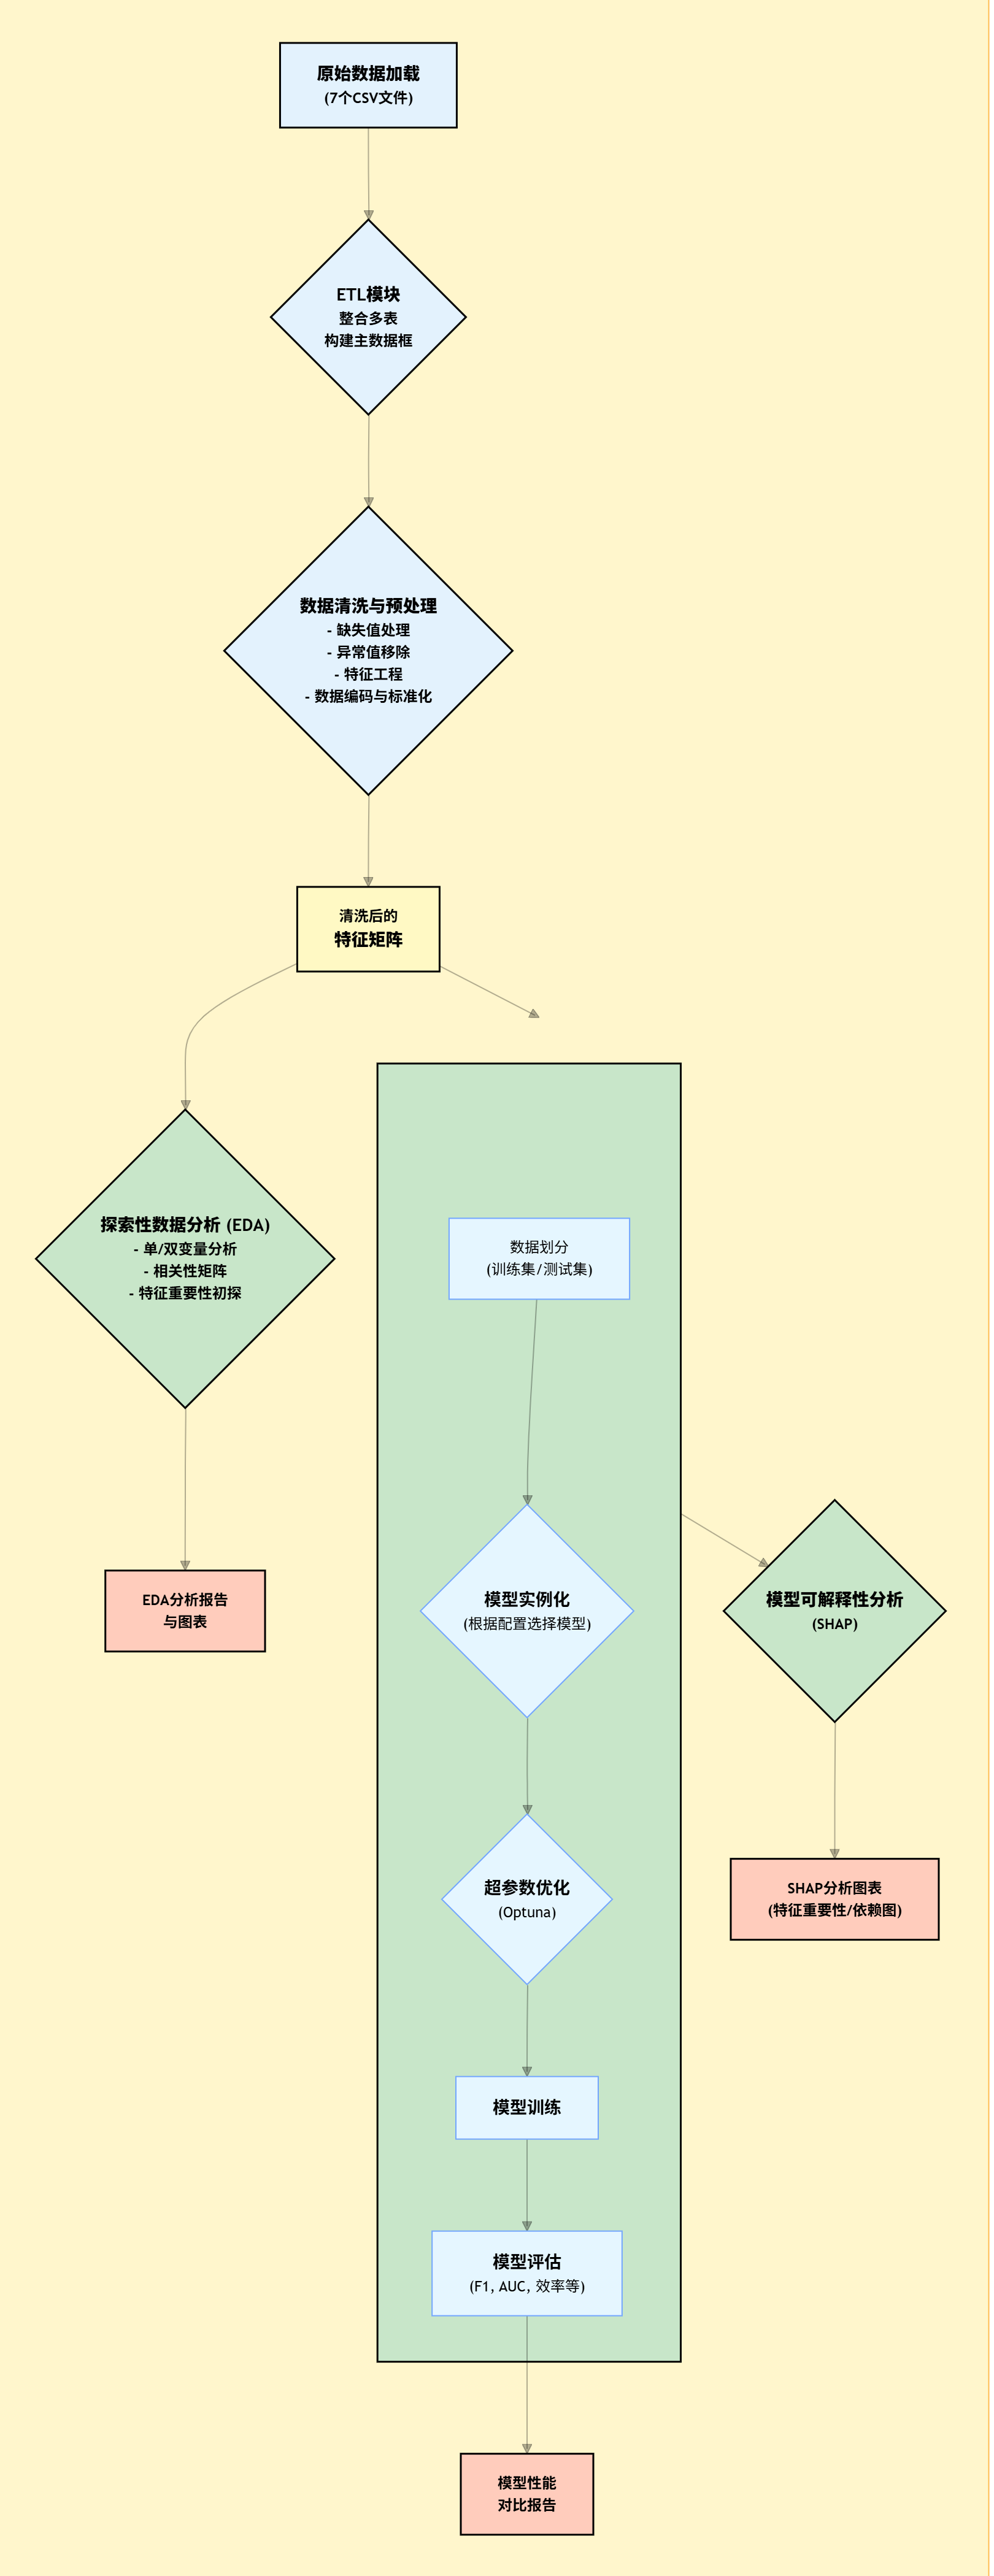
\includegraphics[width=0.5\textwidth]{figures/pipeline.png}
    \caption{系统总体设计流程图}
    \label{fig:pipeline}
\end{figure}


\subsection{数据处理模块}
\begin{itemize}
    \item \textbf{ETL (Extract, Transform, Load):} 该模块负责从原始CSV文件中加载数据，并将多个数据表（如学生信息、注册信息、VLE点击流等）整合成一个包含丰富特征的主数据框。
    \item \textbf{数据清洗:} 实现了缺失值处理（填充或删除）、异常值处理（基于百分位或Z-score）和重复值删除等功能，保证了数据质量。
    \item \textbf{特征工程:} 基于原始数据，构建了一系列具有业务意义的新特征，例如：学习活跃度、VLE交互多样性、成绩变化趋势等。这些高质量特征是提升模型性能的关键。
    \item \par
    本项目的特征工程核心在于对学生与虚拟学习环境（VLE）交互的原始点击流数据进行深度加工和提炼。原始的VLE数据是稀疏且庞大的，我们通过以下步骤将其转化为对模型有价值的结构化特征：
    \begin{itemize}
        \item \textbf{VLE活动聚合：} 我们将学生在VLE中不同类型活动展开为独立的特征，并且对每个活动的点击次数进行聚合统计（构造出n\_days\_和svg\_sum\_clicks\_开头的特征），同时对整个VLE活动也进行整体的统计（构造出learning\_indensity、total\_n\_days等指标）。将原本离散的点击行为，转化为衡量学生在各类学习资源上投入程度的连续特征。
        \item \textbf{关键学业指标构建：} 我们特别关注学生的学业表现。通过整合studentAssessment和assessments表，我们计算了学生在当前时间点前的所有已完成评估的加权平均分，记为 final\_score\_current。这个特征是预测学生最终学业成果的最重要指标之一。
    \end{itemize}
    这些基于领域知识构建的高质量特征，是提升模型预测性能的关键。
    \item \textbf{数据编码与标准化:} 为了使不同尺度的特征能够在模型中公平地发挥作用，并满足许多算法（如SVM）对数据分布的要求，我们对数值型和分类型变量进行了精细化处理：
    \begin{itemize}
        \item \textbf{分类变量处理:} 我们首先识别出所有非数值类型的分类特征（如\texttt{gender}, \texttt{region}, \texttt{highest\_education}等）。为了避免引入序数关系，我们采用\textbf{独热编码（One-Hot Encoding）}进行处理。对于基数（cardinality）非常高的特征，为防止维度爆炸，我们将出现频率较低的类别合并为统一的“Other”类别，然后再进行独热编码。这一过程通过调用pandas库的\texttt{get\_dummies}函数实现。
        \item \textbf{数值变量处理:} 对于所有的数值型特征（如\texttt{studied\_credits}, VLE点击次数，考试分数等），我们采用\textbf{Z-Score标准化（Standardization）}。该方法将每个特征的数据转换成均值为0、标准差为1的分布。这不仅消除了量纲差异，还有助于加速梯度下降等算法的收敛速度。这一过程通过调用scikit-learn库的\texttt{StandardScaler}实现。
    \end{itemize}
\end{itemize}

\subsection{EDA模块}
探索性数据分析（EDA）模块负责对清洗后的数据进行深入分析，以洞察数据分布、特征关系和潜在模式。该模块能够自动生成：
\begin{itemize}
    \item 单变量分布图（直方图、计数图）
    \item 双变量关系图（散点图、箱线图）
    \item 相关性矩阵热力图
    \item 基于随机森林的初步特征重要性排序
\end{itemize}
EDA的发现为后续的建模提供了重要指导。

\subsection{模型训练与评估模块}
这是系统的核心模块，我们设计了一个统一的BaseModel基类，所有具体的模型类都继承自该基类。这种设计保证了所有模型都遵循统一的接口和流程：train, predict, evaluate, save\_model。
\begin{itemize}
    \item \textbf{模型工厂:} 通过一个模型工厂，可以根据配置文件中的名称动态地创建和加载相应的模型实例，实现了系统的插件化和可扩展性。
    \item \textbf{统一评估指标:} 所有模型都采用统一的评估指标，包括准确率、精确率、召回率、F1分数和AUC值，确保了模型比较的公平性。
    \item \textbf{性能监控:} 除了准确性指标，系统还会自动记录每个模型的训练时间、预测时间和模型文件大小，为效率评估提供依据。
\end{itemize}

\section{实验与结果分析}
\subsection{实验设置}
\begin{itemize}
    \item \textbf{硬件环境:} [12th Gen Intel(R) Core(TM) i7-12700H @ 2.30 GHz, 16GB RAM, NVIDIA GeForce RTX 3050 Laptop GPU]
    \item \textbf{软件环境:} Python 3.10, scikit-learn \cite{pedregosa2011scikit}, pandas, Optuna, SHAP
    \item \textbf{数据集划分:} 采用80\%的数据作为训练集，20\%作为测试集，并进行分层抽样以保证训练集和测试集中目标变量的分布一致。
    \item \textbf{超参数优化:} 对所有模型均使用Optuna进行20次迭代的超参数搜索，优化目标为交叉验证的F1分数。
\end{itemize}

\subsection{EDA关键发现}
\begin{figure}[!htbp]
    \centering
    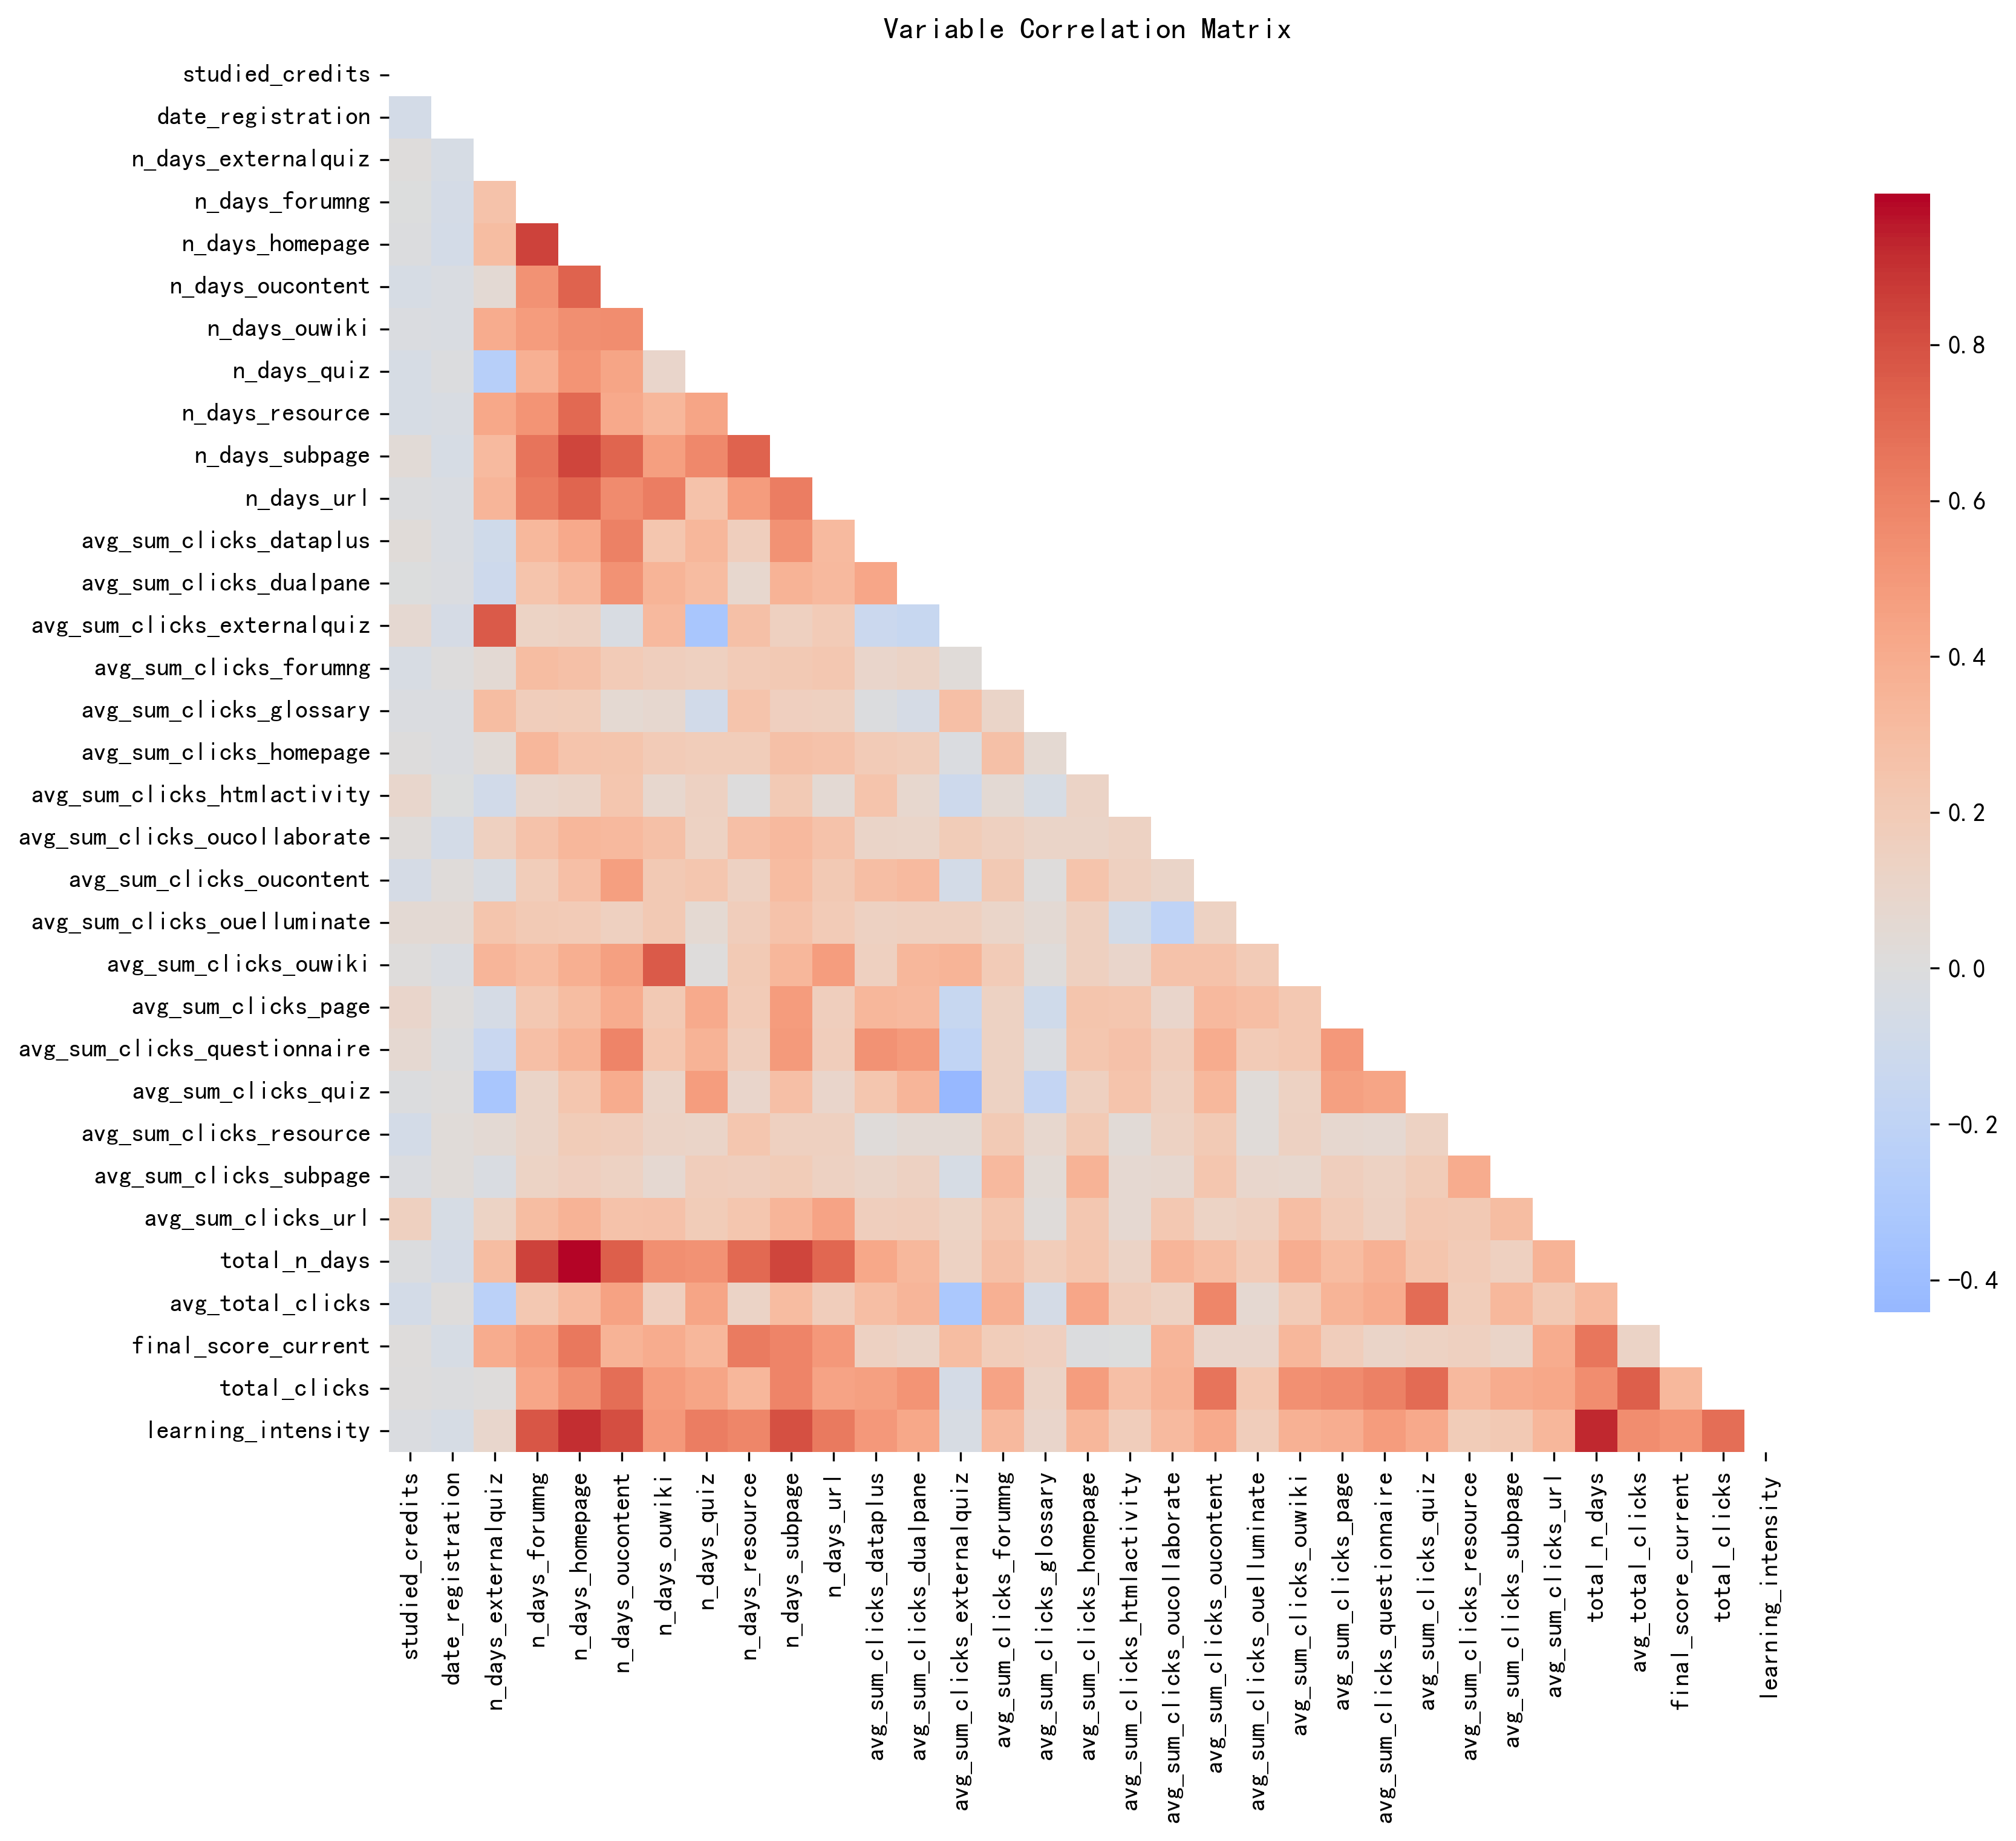
\includegraphics[width=0.5\textwidth]{figures/correlation_matrix.png}
    \caption{数值变量特征相关性矩阵热力图}
    \label{fig:cm}
\end{figure}

\begin{figure}[!htbp]
    \centering
    \begin{minipage}[t]{0.32\textwidth}
        \centering
        \includegraphics[width=\textwidth]{figures/numeric_distributions.png}
        \caption{数值变量分布图}
        \label{fig:numeric_distributions}
    \end{minipage}
    \hfill
    \begin{minipage}[t]{0.32\textwidth}
        \centering
        \includegraphics[width=0.8\textwidth]{figures/numeric_vs_target.png}
        \caption{数值变量与目标变量的双变量分析}
        \label{fig:numeric_vs_target}
    \end{minipage}
    \hfill
    \begin{minipage}[t]{0.32\textwidth}
        \centering
        \includegraphics[width=0.5\textwidth]{figures/categorical_vs_target.png}
        \caption{分类变量与目标变量的双变量分析}
        \label{fig:categorical_vs_target}
    \end{minipage}
    \caption{EDA分析}
    \label{fig:overall}
\end{figure}

通过EDA分析，通过数值变量特征相关性矩阵热力图。我们发现整体来说，各个特征之间的相关性并不大，vle的两个总体统计特征total\_n\_days和learning\_indensity与某些vle活动类型的聚合特征有较高的相关性。

对于单变量的分析，几乎所有的vle活动特征都右偏斜，这说明大部分学生在VLE上的交互行为较少，只有少部分学生非常活跃。

对于双变量分析，我发现大部分特征在at\_risk=1和at\_risk=0的分布上有明显差异。尤其是在vle活动特征中。

对于分类变量的双变量分析，我们发现某些特征（如region, highest\_education）在at\_risk=1和at\_risk=0之间有显著差异。如n\_days\_oucollaborate和activity\_diversity等特征在两类学生中分布差异明显，说明这些特征对学业风险有较强的区分能力。
\subsection{模型性能对比分析}
\subsubsection{准确性对比}
我们将7个模型在测试集上的核心准确性指标进行了对比，其中SVM准确率为92.25\%,随机森林为92.15\%,逻辑回归为90.40\%,决策树为91.75\%。调整兰德指数kmeans为0.089，em为0.033。从结果可以看出，随机森林、SVM在准确率上表现最佳。
这是正常的，相比于线性的逻辑回归，SVM可以拟合非线性关系，而随机森林由多个决策树组成，通过 bagging（自助采样）和特征随机选择训练，每棵树独立预测，最后通过多数投票（分类）或平均（回归）得出结果。
相比于决策树的稳定性差，抗过拟合能力强，鲁棒性高，适用于大规模数据集，能够处理高维特征和复杂的非线性关系。
对这种多特征，大数据集的分类问题，随机森林无疑会表现更加优异。
而K-Means和高斯混合模型由于任务性质差异，表现相对较弱。

在F1分数和AUC方面，各模型表现和准确率相似，随机森林和SVM依旧表现较优。逻辑回归和决策树的F1分数略低，但仍然在可接受范围内。

\begin{table}[!htbp]
    \centering
    \caption{各监督学习模型准确性指标对比}
    \label{tab:accuracy}
    \resizebox{\textwidth}{!}{%
    \begin{tabular}{l|ccccc}
        \toprule
        \textbf{模型} & \textbf{准确率 (Accuracy)} & \textbf{精确率 (Precision)} & \textbf{召回率 (Recall)} & \textbf{F1 分数 (F1-Score)} & \textbf{AUC} \\
        \midrule
        随机森林 & 0.9215 & 0.9246 & 0.9215 & 0.9211 & 0.9713 \\
        支持向量机 (SVM) & 0.9225 & 0.9240 & 0.9225 & 0.9223 & 0.9701 \\
        决策树 & 0.9177 & 0.9179 & 0.9177 & 0.9176 & 0.9686 \\
        逻辑回归 & 0.9039 & 0.9043 & 0.9039 & 0.9037 & 0.9650 \\
        \bottomrule
    \end{tabular}%
    }
\end{table}

\begin{table}[!htbp]
    \centering
    \caption{各模型效率与聚类性能指标对比}
    \label{tab:efficiency}
    \resizebox{\textwidth}{!}{%
    \begin{tabular}{l|cc|c}
        \toprule
        \textbf{模型} & \textbf{训练时间 (秒)} & \textbf{预测时间 (秒)} & \textbf{调整兰德指数 (ARI)} \\
        \midrule
        支持向量机 (SVM) & 2777.22 & 4.817  & - \\
        K-Means & 117.40 & < 0.01  & 0.0895 \\
        随机森林 & 59.91 & < 0.01  & - \\
        逻辑回归 & 17.42 & < 0.01  & - \\
        高斯混合模型 (EM) & 17.47 & 0.017  & 0.0332 \\
        决策树 & 13.62 & < 0.01  & - \\
        \bottomrule
    \end{tabular}%
    }
\end{table}

\subsubsection{随机森林和决策树的对比}
随机森林（Random Forest）作为一种集成学习（Ensemble Learning）的代表性算法，其设计初衷正是为了克服单个决策树（Decision Tree）的固有缺陷。决策树以其白盒特性、符合人类直觉的决策逻辑而备受青睐，但其致命弱点在于对训练数据中的微小扰动极为敏感，容易产生过拟合，导致泛化能力不佳。随机森林通过引入“双重随机性”——自助采样（Bootstrap Aggregating, or Bagging）和特征随机选择——构建了一个由多棵决策树组成的“森林”，并通过集体投票或取平均的方式进行最终决策，从而显著提升了模型的稳定性和准确性。本节将从准确性、效率、鲁棒性与参数敏感度、可解释性四个维度，对这两种模型进行深入的比较分析。

\textbf{准确性与抗过拟合能力：}
从\ref{tab:accuracy}中的数据可以看出，随机森林在所有关键准确性指标上均略优于单一决策树。随机森林的准确率为92.15\%，F1分数为0.9211，AUC为0.9713；而决策树的对应指标分别为91.77\%，0.9176和0.9686。尽管在数值上的领先幅度不大，但这背后揭示了两种模型在泛化能力上的本质差异，而这种差异的根源在于对“过拟合”的控制。

决策树的构建过程是一个“贪心”算法，它在每个节点都试图找到当前最优的特征分裂，以便最大程度地“纯化”子节点。这个过程使得决策树对训练数据中的细节和噪声异常敏感，非常容易产生高方差（variance），即过拟合倾向。这种内在机制在\ref{fig:dt_boundary}的决策边界图上得到了直观的体现。图中清晰的、与坐标轴平行的“阶梯状”边界，正是决策树这种轴对齐分裂规则的必然结果。虽然这个边界本身不直接等同于过拟合，但它揭示了模型对训练样本分布的精细“雕刻”，这种高度的依赖性使其在新数据上的表现变得不稳定。

相比之下，随机森林通过“双重随机性”构建了一个由数百棵“各不相同”的决策树组成的集成模型。\ref{fig:rf_boundary}中随机森林的决策边界之所以更加平滑、有机，正是因为它是由成百上千个不同的“阶梯状”边界投票、平均而成的。这个平均过程极大地降低了模型的方差，平滑了单个决策树对训练数据中特定噪声或异常点的敏感性，使其能够更好地捕捉数据的整体趋势而非局部波动。因此，测试集上更高的准确率指标，正是对随机森林模型泛化能力更强的有力数据佐证，也从结果上验证了其对单一决策树过拟合倾向的有效抑制。

\begin{figure}[!htbp]
    \centering
    \begin{minipage}[t]{0.48\textwidth}
        \centering
        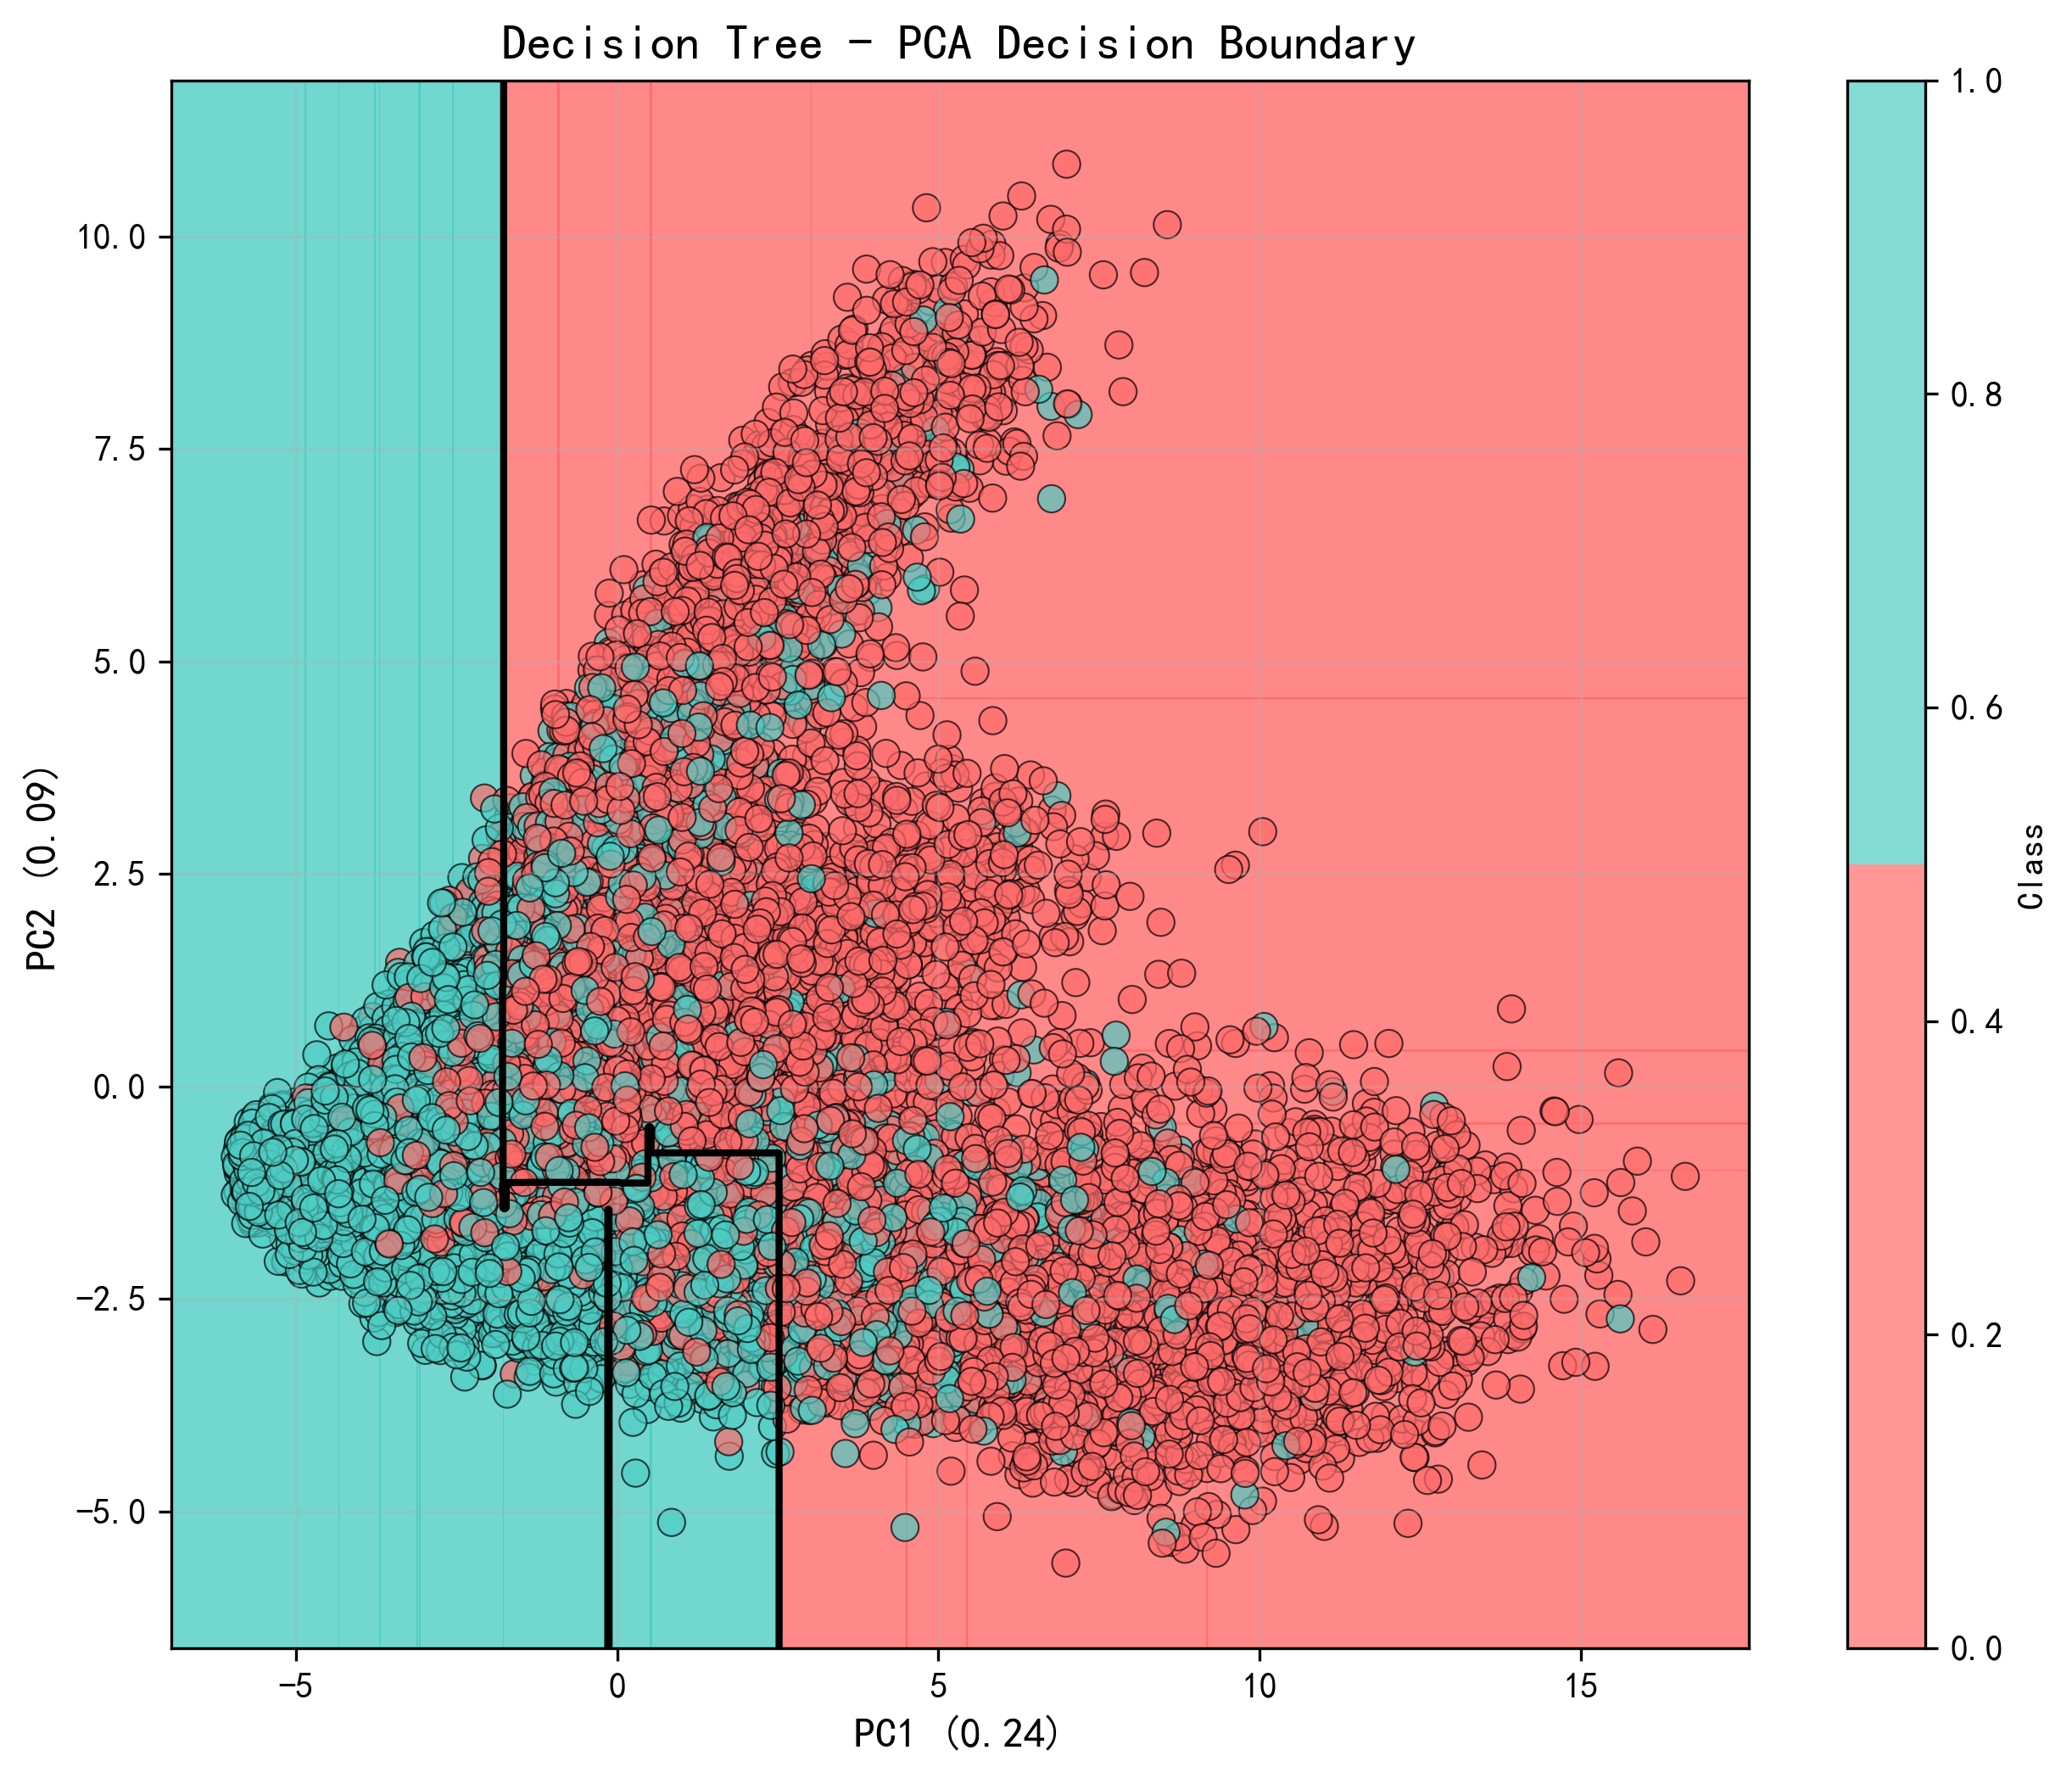
\includegraphics[width=\textwidth]{figures/decision_tree_pca_decision_boundary.png}
        \caption{决策树决策边界}
        \label{fig:dt_boundary}
    \end{minipage}
    \hfill
    \begin{minipage}[t]{0.48\textwidth}
        \centering
        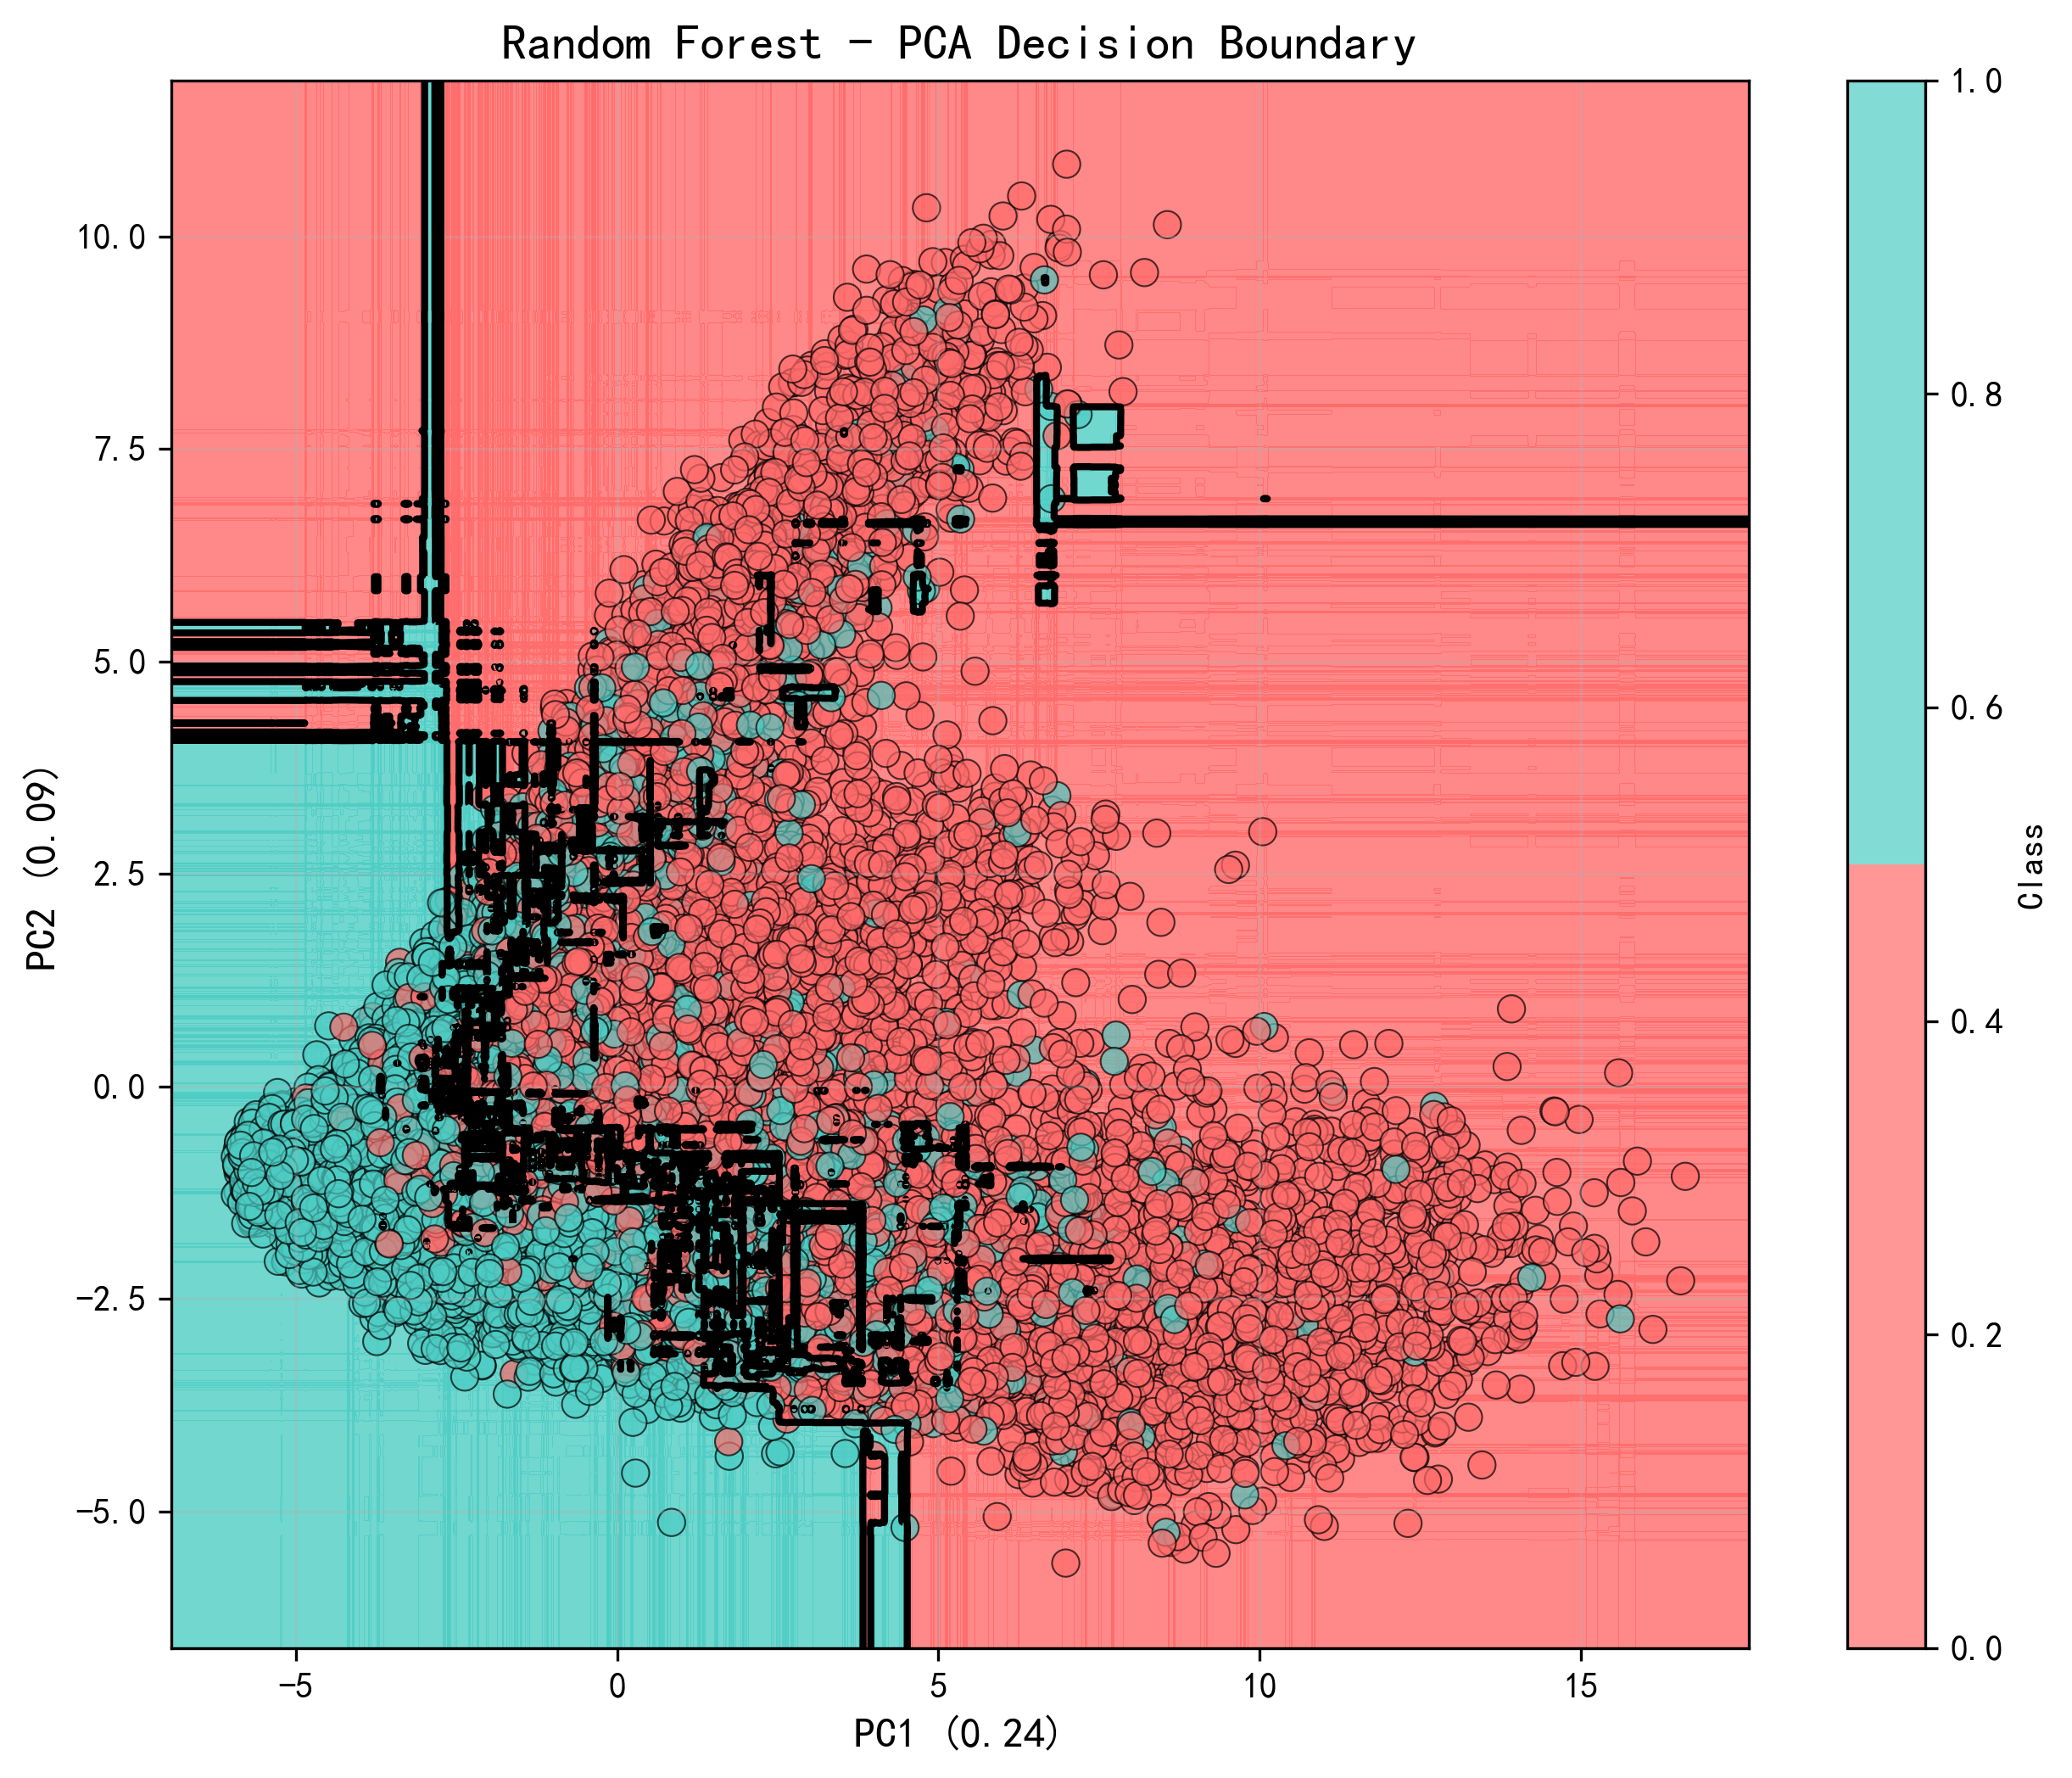
\includegraphics[width=\textwidth]{figures/random_forest_pca_decision_boundary.png}
        \caption{随机森林决策边界}
        \label{fig:rf_boundary}
    \end{minipage}
    \caption{决策树与随机森林决策边界对比（PCA降维）}
    \label{fig:dt_rf_boundaries}
\end{figure}

\textbf{效率对比：}
效率是决策树相比随机森林最显著的优势。根据\ref{tab:efficiency}的数据，训练一个决策树模型仅需13.62秒，而训练随机森林则需要59.91秒，是前者的4倍多。这种差异是完全符合预期的：随机森林需要独立构建并训练数百棵决策树（本项目中n\_estimators优化后为200），其计算成本自然与树的数量成正比。在预测阶段，虽然随机森林也需要聚合多棵树的结果，但由于现代计算库的并行优化，其预测时间依然极快。因此，在对模型训练速度有严苛要求、需要快速验证迭代的场景，或者在计算资源极其有限的环境下，单一决策树可能是更务实的选择。

\textbf{鲁棒性与参数敏感度：}
鲁棒性是随机森林的另一大强项。由于Bagging机制，随机森林对数据集中的噪声和异常值不敏感，个别异常点很难对整个森林的决策产生决定性影响。相反，单一决策树则可能为了拟合一个异常点而生长出不必要的分支。在参数调优方面，虽然随机森林的超参数更多（如n\_estimators, max\_features），但它通常对单个超参数的敏感度低于决策树。对于决策树，max\_depth或min\_samples\_leaf等剪枝参数的选择至关重要，设置不当极易导致过拟合或欠拟合。而随机森林中，由于集成的平均效应，单棵树即便有些许过拟合，其影响也会被其他树中和。通常只需将树的数量（n\_estimators）设置得足够大，模型性能就会趋于稳定，这使得随机森林的调参过程相对更为简单和鲁棒。

\textbf{可解释性：}
可解释性是决策树胜过随机森林的维度，也是两者最核心的权衡点（Trade-off）。决策树的决策过程完全透明，可以轻松地可视化成一棵树状图（如图\ref{fig:d}所示），我们可以清晰地追踪任何一个样本从根节点到叶节点的完整决策路径。这种“白盒”特性在许多需要向业务方解释模型逻辑的领域（如金融风控、医疗诊断）是至关重要的。相比之下，随机森林是一个典型的“黑箱”模型。我们无法得知数百棵树是如何共同作用得出最终结果的。然而，正如项目中所述，我们可以借助SHAP等模型事后解释工具来弥补这一缺陷。通过SHAP摘要图，我们依然可以了解哪些特征在全局上对模型最重要，其重要性甚至比单一决策树提供的特征重要性度量（如Gini importance）更为可靠。

综上所述，决策树与随机森林的选择是一个典型的“性能与可解释性”的权衡。当任务目标是追求极致的预测精度和模型稳定性时，随机森林无疑是更优的选择。而当业务需求强调模型决策过程的透明度与可解释性，或者计算资源极为有限时，一个经过良好剪枝的决策树则更具优势。


\begin{figure}[!htbp]
    \centering
    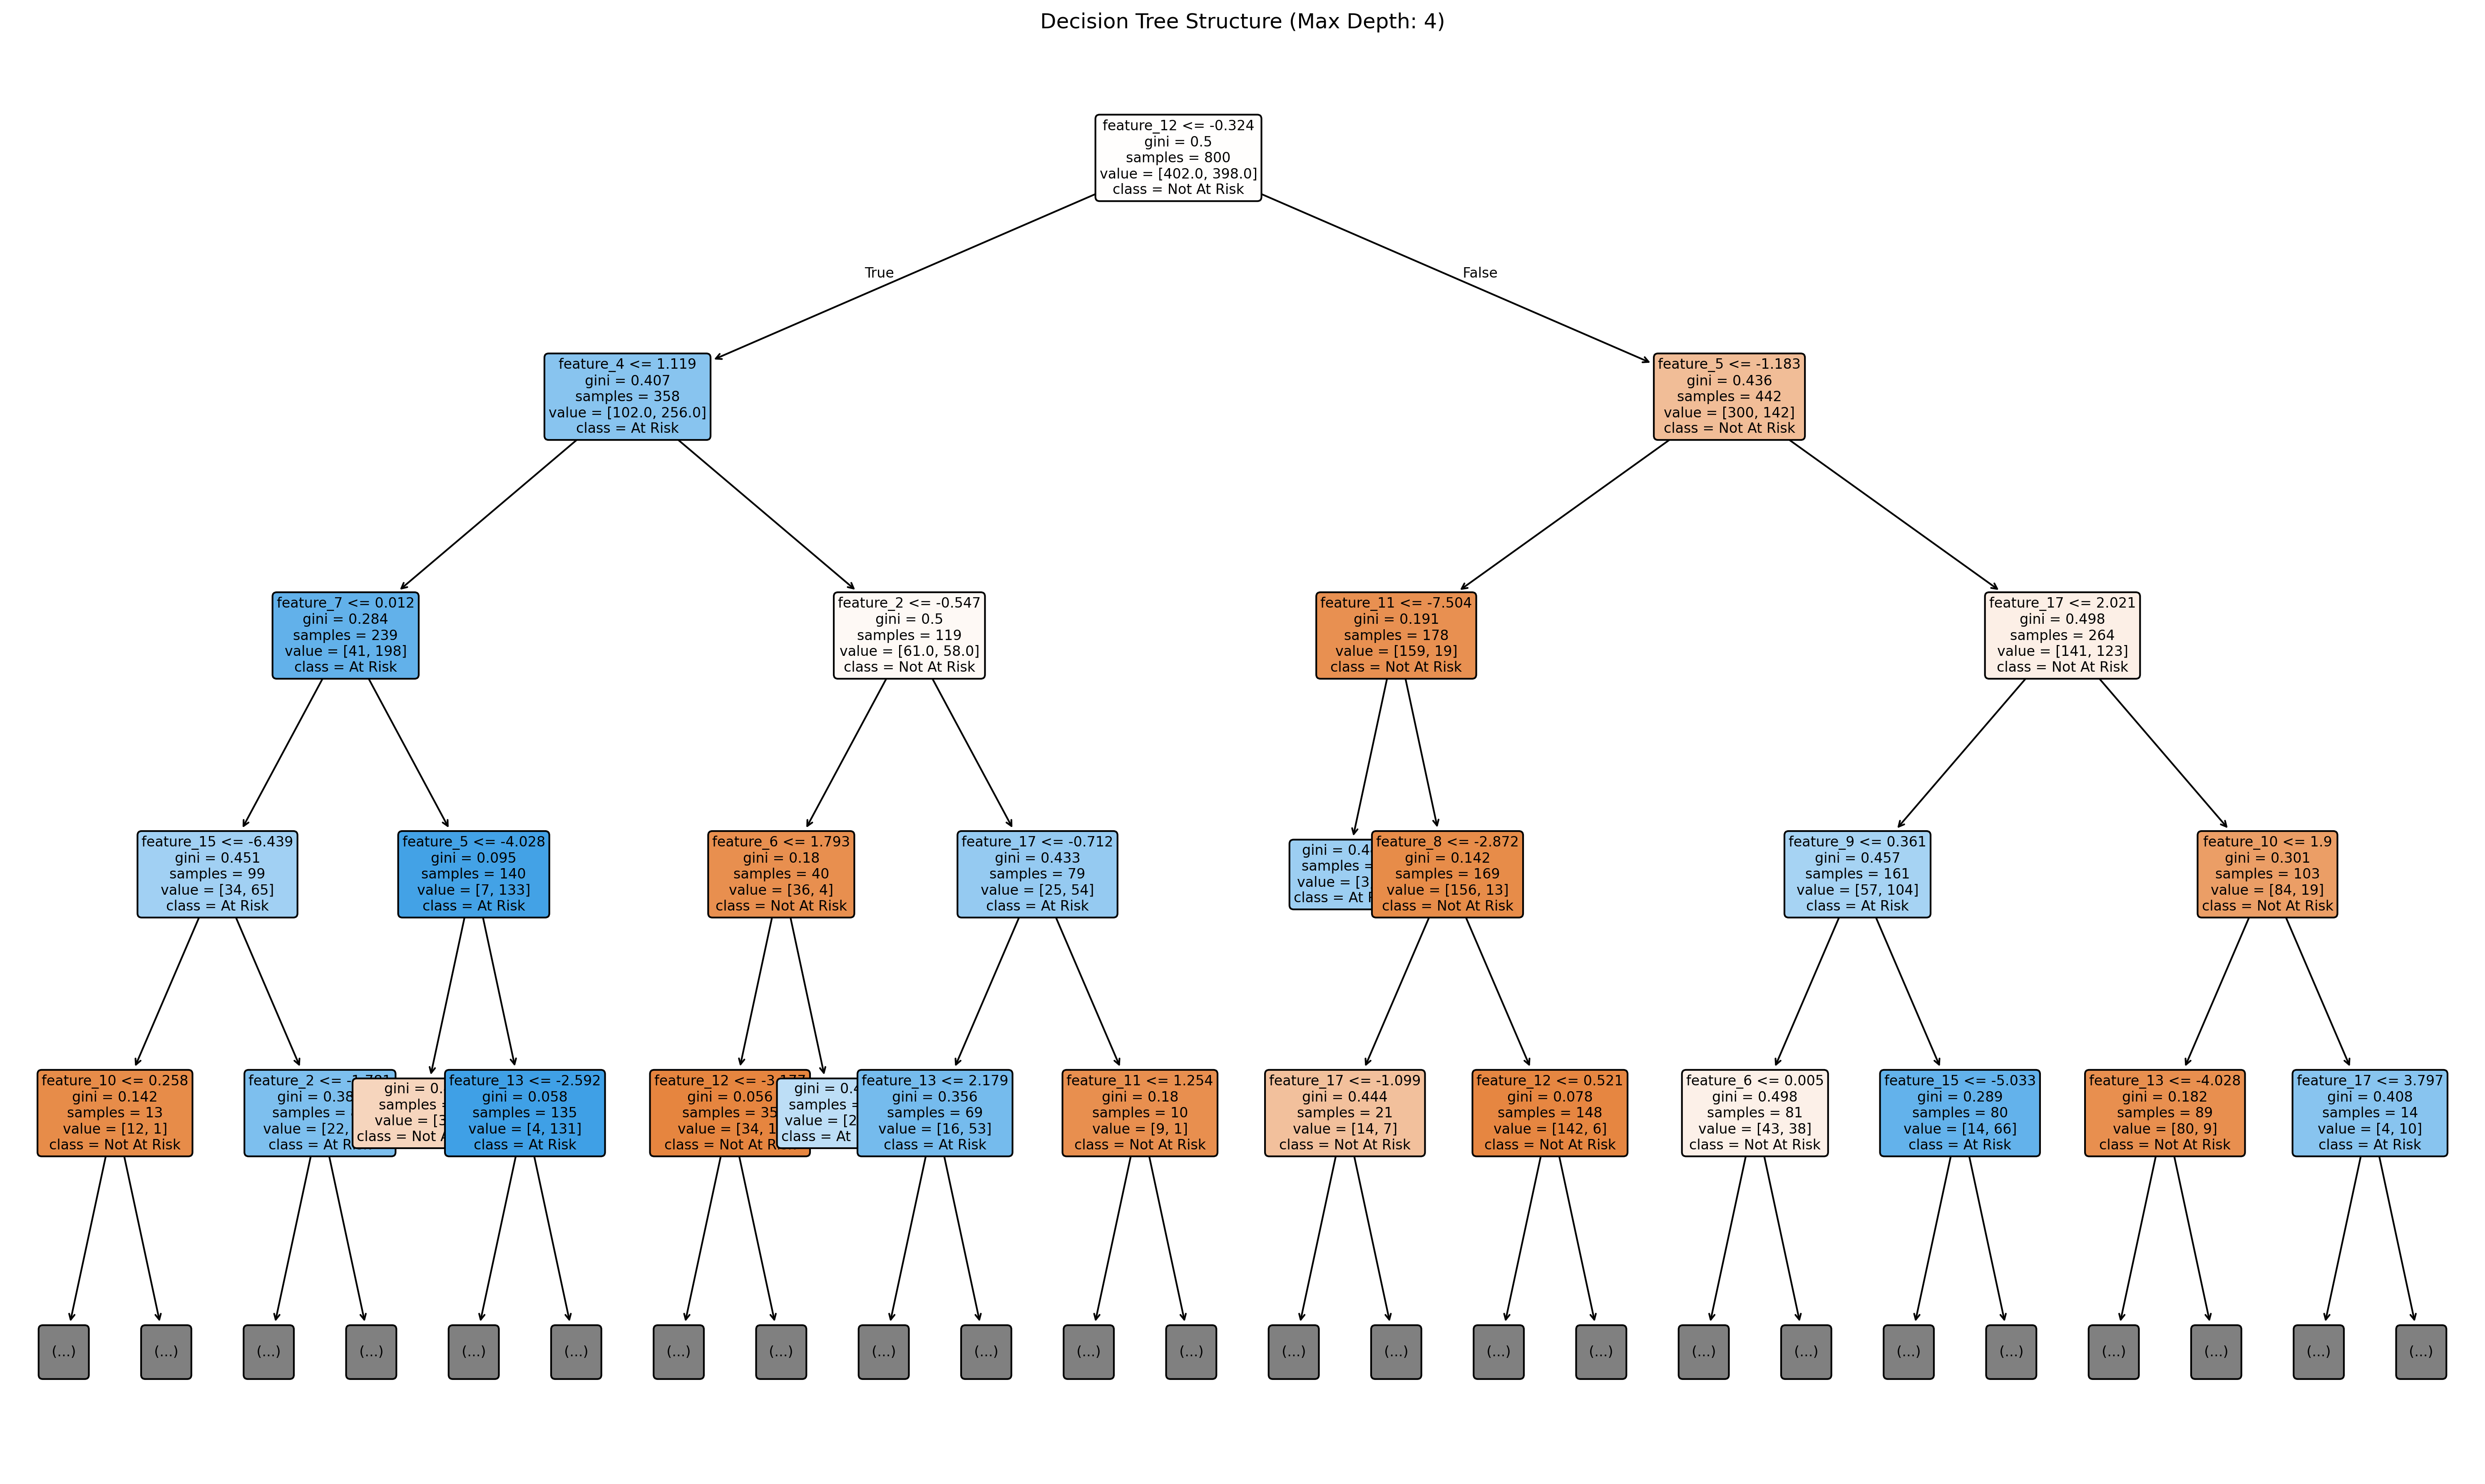
\includegraphics[width=0.5\textwidth]{figures/decisiontreemodeler_tree_structure.png}
    \caption{本项目生成的决策树结构图}
    \label{fig:d}
\end{figure}

\subsubsection{逻辑回归和SVM的对比}
逻辑回归（Logistic Regression）与支持向量机（Support Vector Machine, SVM）是机器学习分类领域中最经典、最强大的两种算法。逻辑回归作为广义线性模型的代表，以其简洁、高效、易于解释的特点，成为众多分类问题的首选基准。而SVM则通过引入核技巧（Kernel Trick）和最大间隔（Max-margin）思想，在高维和非线性问题上展现出卓越的性能。本项目中，逻辑回归的决策边界是线性的，而SVM我们采用了高斯核（RBF），使其能够学习非线性的决策边界。本节将依据详实的实验数据，从准确性、效率、鲁棒性与参数敏感度、可解释性四个方面，对二者进行全面深入的比较。

\textbf{准确性与决策边界：}
根据\ref{tab:accuracy}，SVM在各项准确性指标上全面优于逻辑回归。SVM的准确率、F1分数和AUC分别为92.25\%、0.9223和0.9701，而逻辑回归则为90.39\%、0.9037和0.9650。这一结果充分说明，在本次学业风险预测任务中，数据特征与目标变量之间存在显著的非线性关系。从\ref{fig:svmlogistic}中已经展示的决策边界对比图可以直观地印证这一点。逻辑回归（\ref{fig:logistic}）尽力寻找一个最优的线性超平面来分割数据，但其线性假设的局限性使其无法完美地分离两个高度交织的类别。相比之下，SVM（\ref{fig:svm}）通过RBF核将数据映射到更高维的空间，成功地学习到了一个复杂的、非线性的决策边界，该边界能够更灵活地包裹和区分“高风险”与“低风险”学生群体，从而取得了更高的分类精度。这表明SVM强大的非线性建模能力是其在本任务中获胜的关键。

\textbf{效率对比：一个数量级的差异}
效率是逻辑回归相比SVM最压倒性的优势，两者的性能开销完全不在一个数量级上。从\ref{tab:efficiency}可以看到，逻辑回归的训练时间仅为17.42秒，而SVM的训练时间高达惊人的2777.22秒（约46分钟），是前者的近160倍。这种巨大的差异源于两者底层优化目标的根本不同。逻辑回归求解的是一个凸优化问题，可以通过梯度下降等高效算法快速找到全局最优解。而SVM求解的是一个二次规划（Quadratic Programming）问题，其计算复杂度与训练样本数量的平方或立方（取决于具体实现）有关。在本项目的数万条样本上，这种高复杂度导致了巨大的时间开销。在预测阶段，SVM也略慢于逻辑回归，因为它需要计算新样本与所有支持向量（Support Vectors）的距离。因此，在任何对训练或预测延迟有要求的工业级应用中，或者在需要频繁重新训练模型的大数据场景下，SVM的计算成本往往是其应用的主要瓶颈，而逻辑回归则展现出无与伦比的效率和可扩展性。

\textbf{鲁棒性与参数敏感度：}
在鲁棒性方面。逻辑回归对所有样本一视同仁，因此对异常值较为敏感，个别远离决策边界的异常点可能会对线性超平面的位置产生显著影响。而SVM的决策边界仅由少数“支持向量”决定，远离边界的样本点对模型没有影响，因此其对异常值具有天然的鲁棒性。然而，在参数敏感度方面，SVM的调参过程通常比逻辑回归更为复杂。逻辑回归的核心超参数主要是正则化强度C。而对于RBF核的SVM，则需要同时优化正则化参数C和核函数宽度gamma。gamma决定了单个样本的影响范围，C则权衡了“最大化间隔”和“最小化分类错误”。这两个参数的组合对模型性能影响巨大，且相互关联，需要通过更精细的搜索（如网格搜索或本项目使用的Optuna）来寻找最优组合，这无疑增加了模型优化的难度。

\textbf{可解释性：}
与决策树和随机森林的对比类似，逻辑回归和SVM之间也存在着“可解释性与性能”的权衡。逻辑回归具有极强的可解释性。其训练出的模型系数（coefficients）直接量化了每个特征对预测结果（的对数几率）的影响。正系数表示该特征增加会提高属于正类的概率，负系数则相反。这种清晰的解释能力使其深受业务分析人员的喜爱。相反，SVM是一个相对的“黑箱”。我们很难直观地理解RBF核在高维空间中是如何工作的，也无法像逻辑回归那样得到每个特征明确的权重。尽管如此，我们依然可以通过SHAP分析来解释SVM的预测。通过对比逻辑回归和SVM的SHAP摘要图（如logisticregressionmodeler\_shap\_summary.png），我们可以发现，尽管两个模型的机制不同，但它们识别出的关键风险预测因子高度一致（如final\_score\_current等），这从侧面印证了模型结论的可靠性。

综上，逻辑回归和SVM代表了两种不同的建模哲学。逻辑回归是速度、简洁和可解释性的典范，是处理大规模、线性可分或需要强解释性任务的理想选择。而SVM则是性能和非线性建模能力的标杆，适用于样本量适中、特征维度高、且数据关系复杂的场景，但使用者必须为其高昂的计算成本和更复杂的调优过程做好准备。

\begin{figure}[!htbp]
    \centering
    \begin{minipage}[t]{0.46\textwidth}
        \centering
        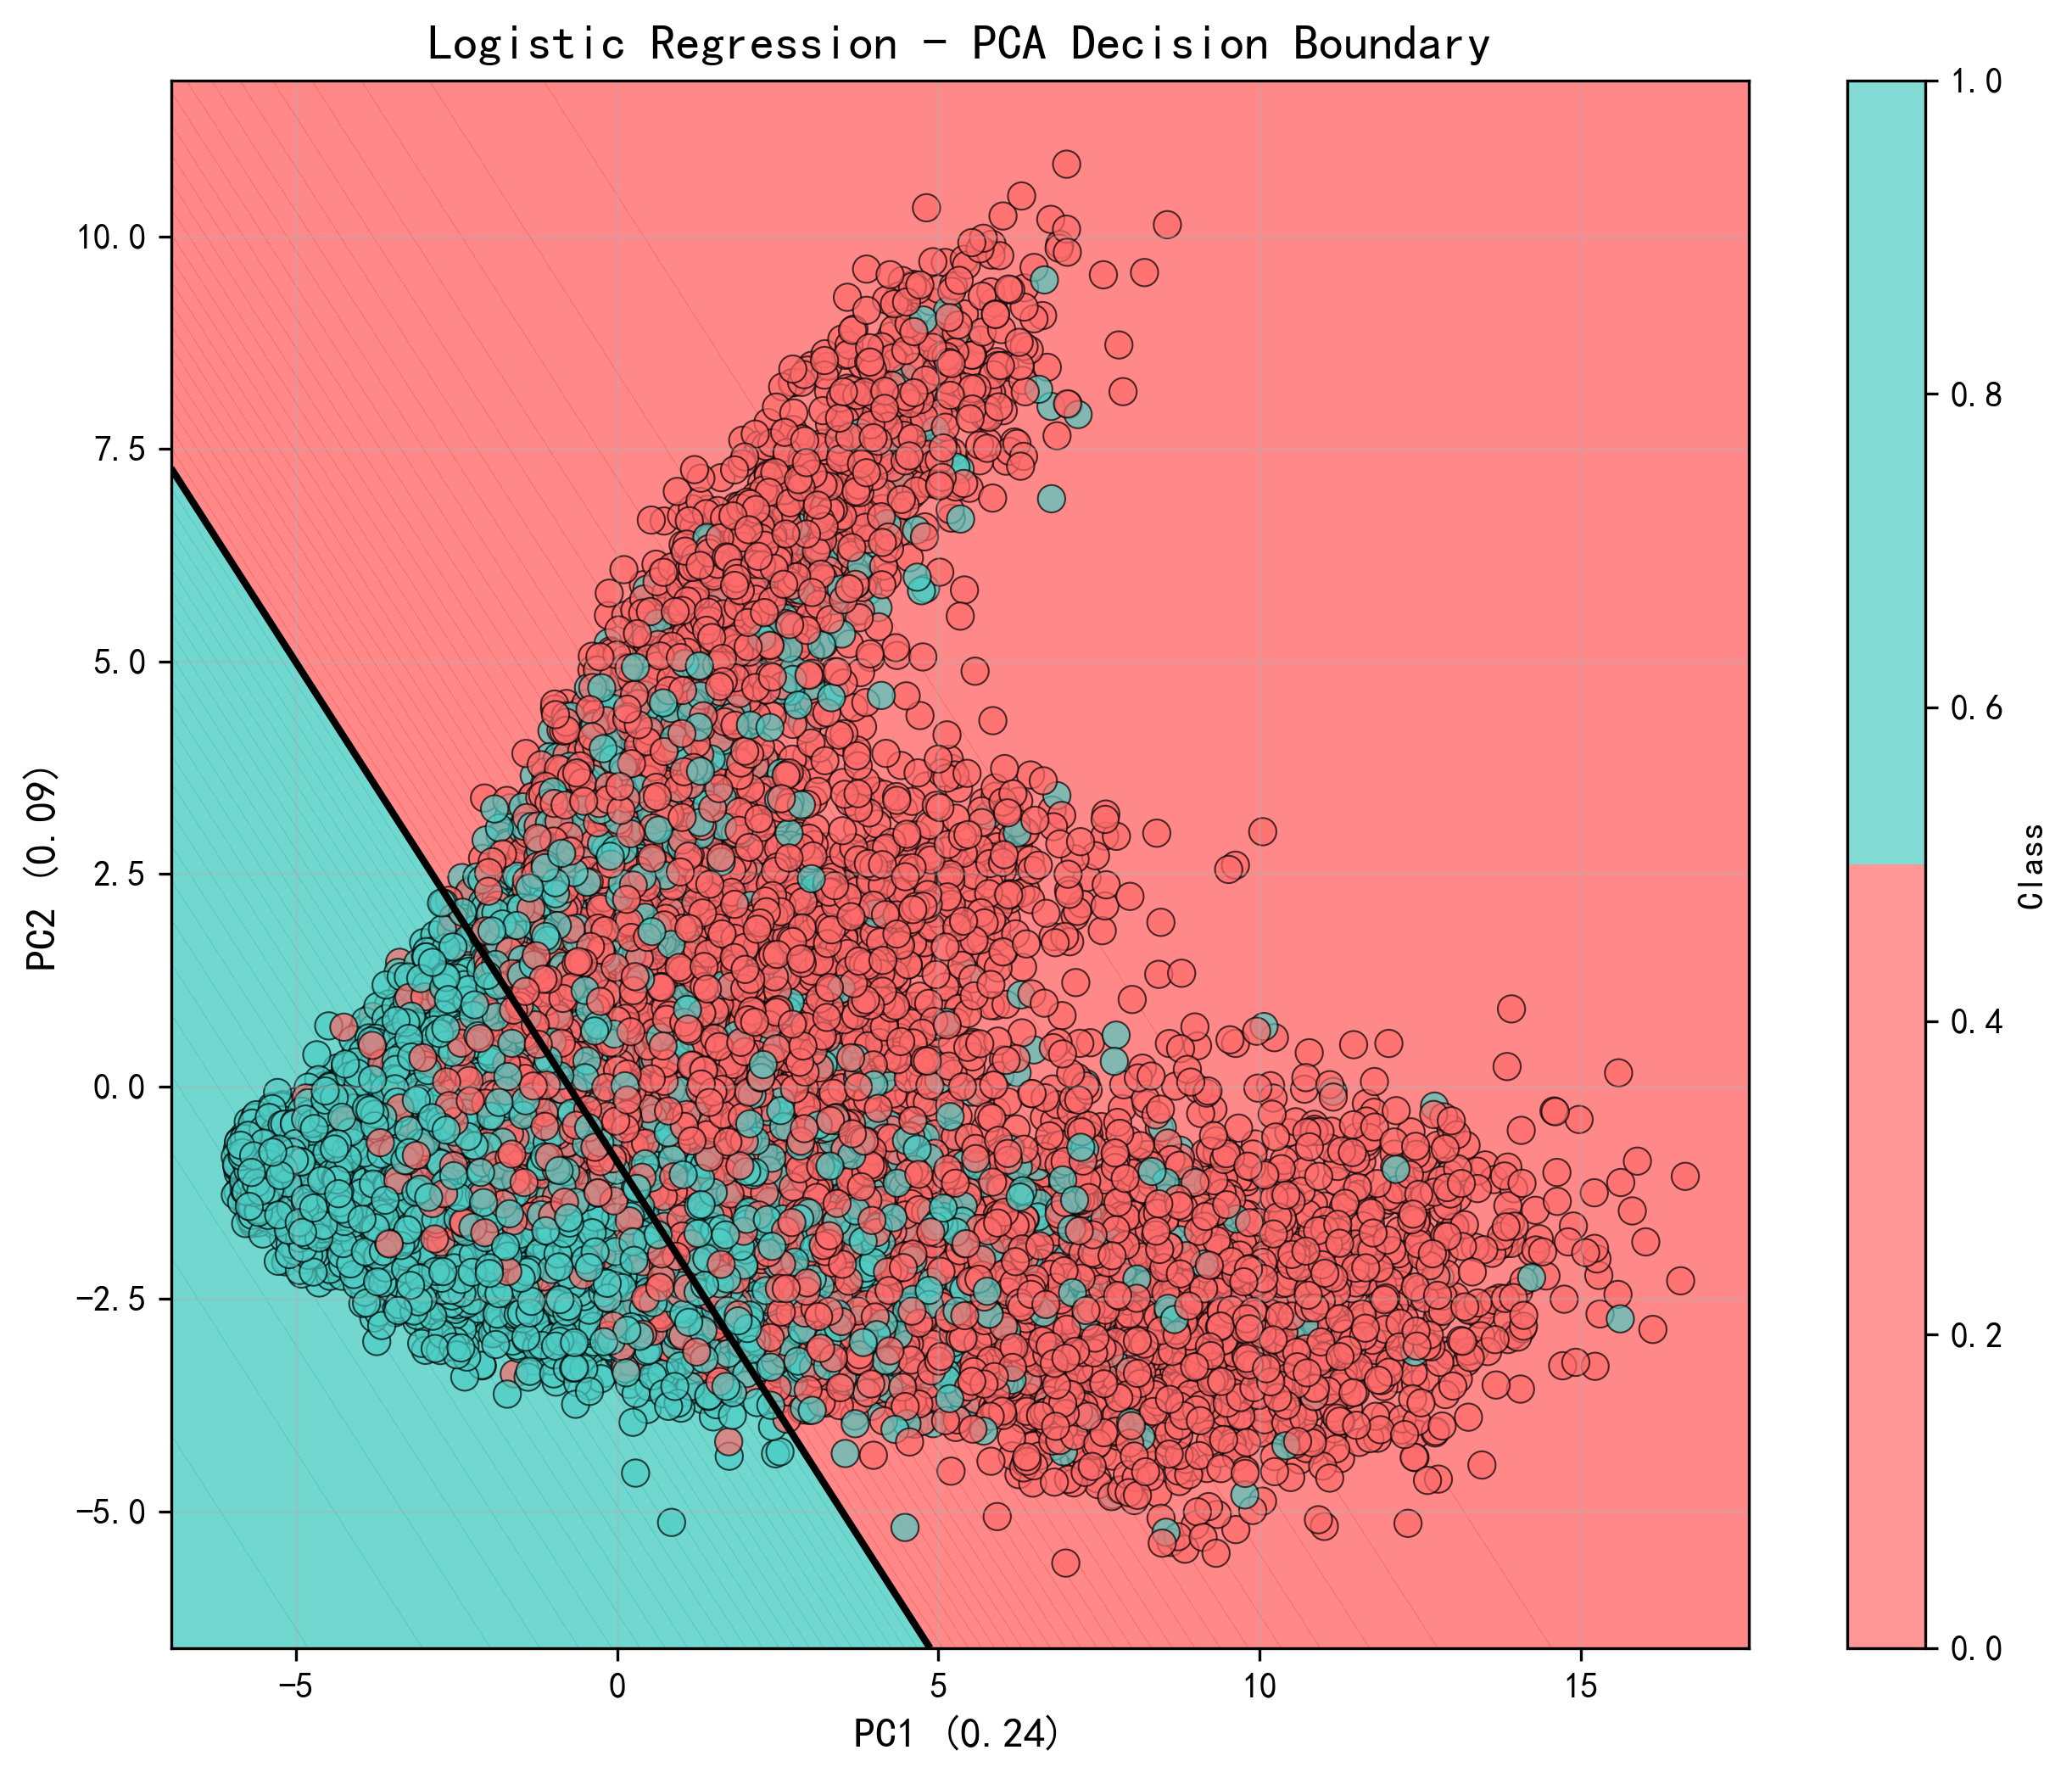
\includegraphics[width=\textwidth]{figures/logistic_regression_pca_decision_boundary.png}
        \caption{逻辑回归决策边界}
        \label{fig:logistic}
    \end{minipage}
    \hfill
    \begin{minipage}[t]{0.46\textwidth}
        \centering
        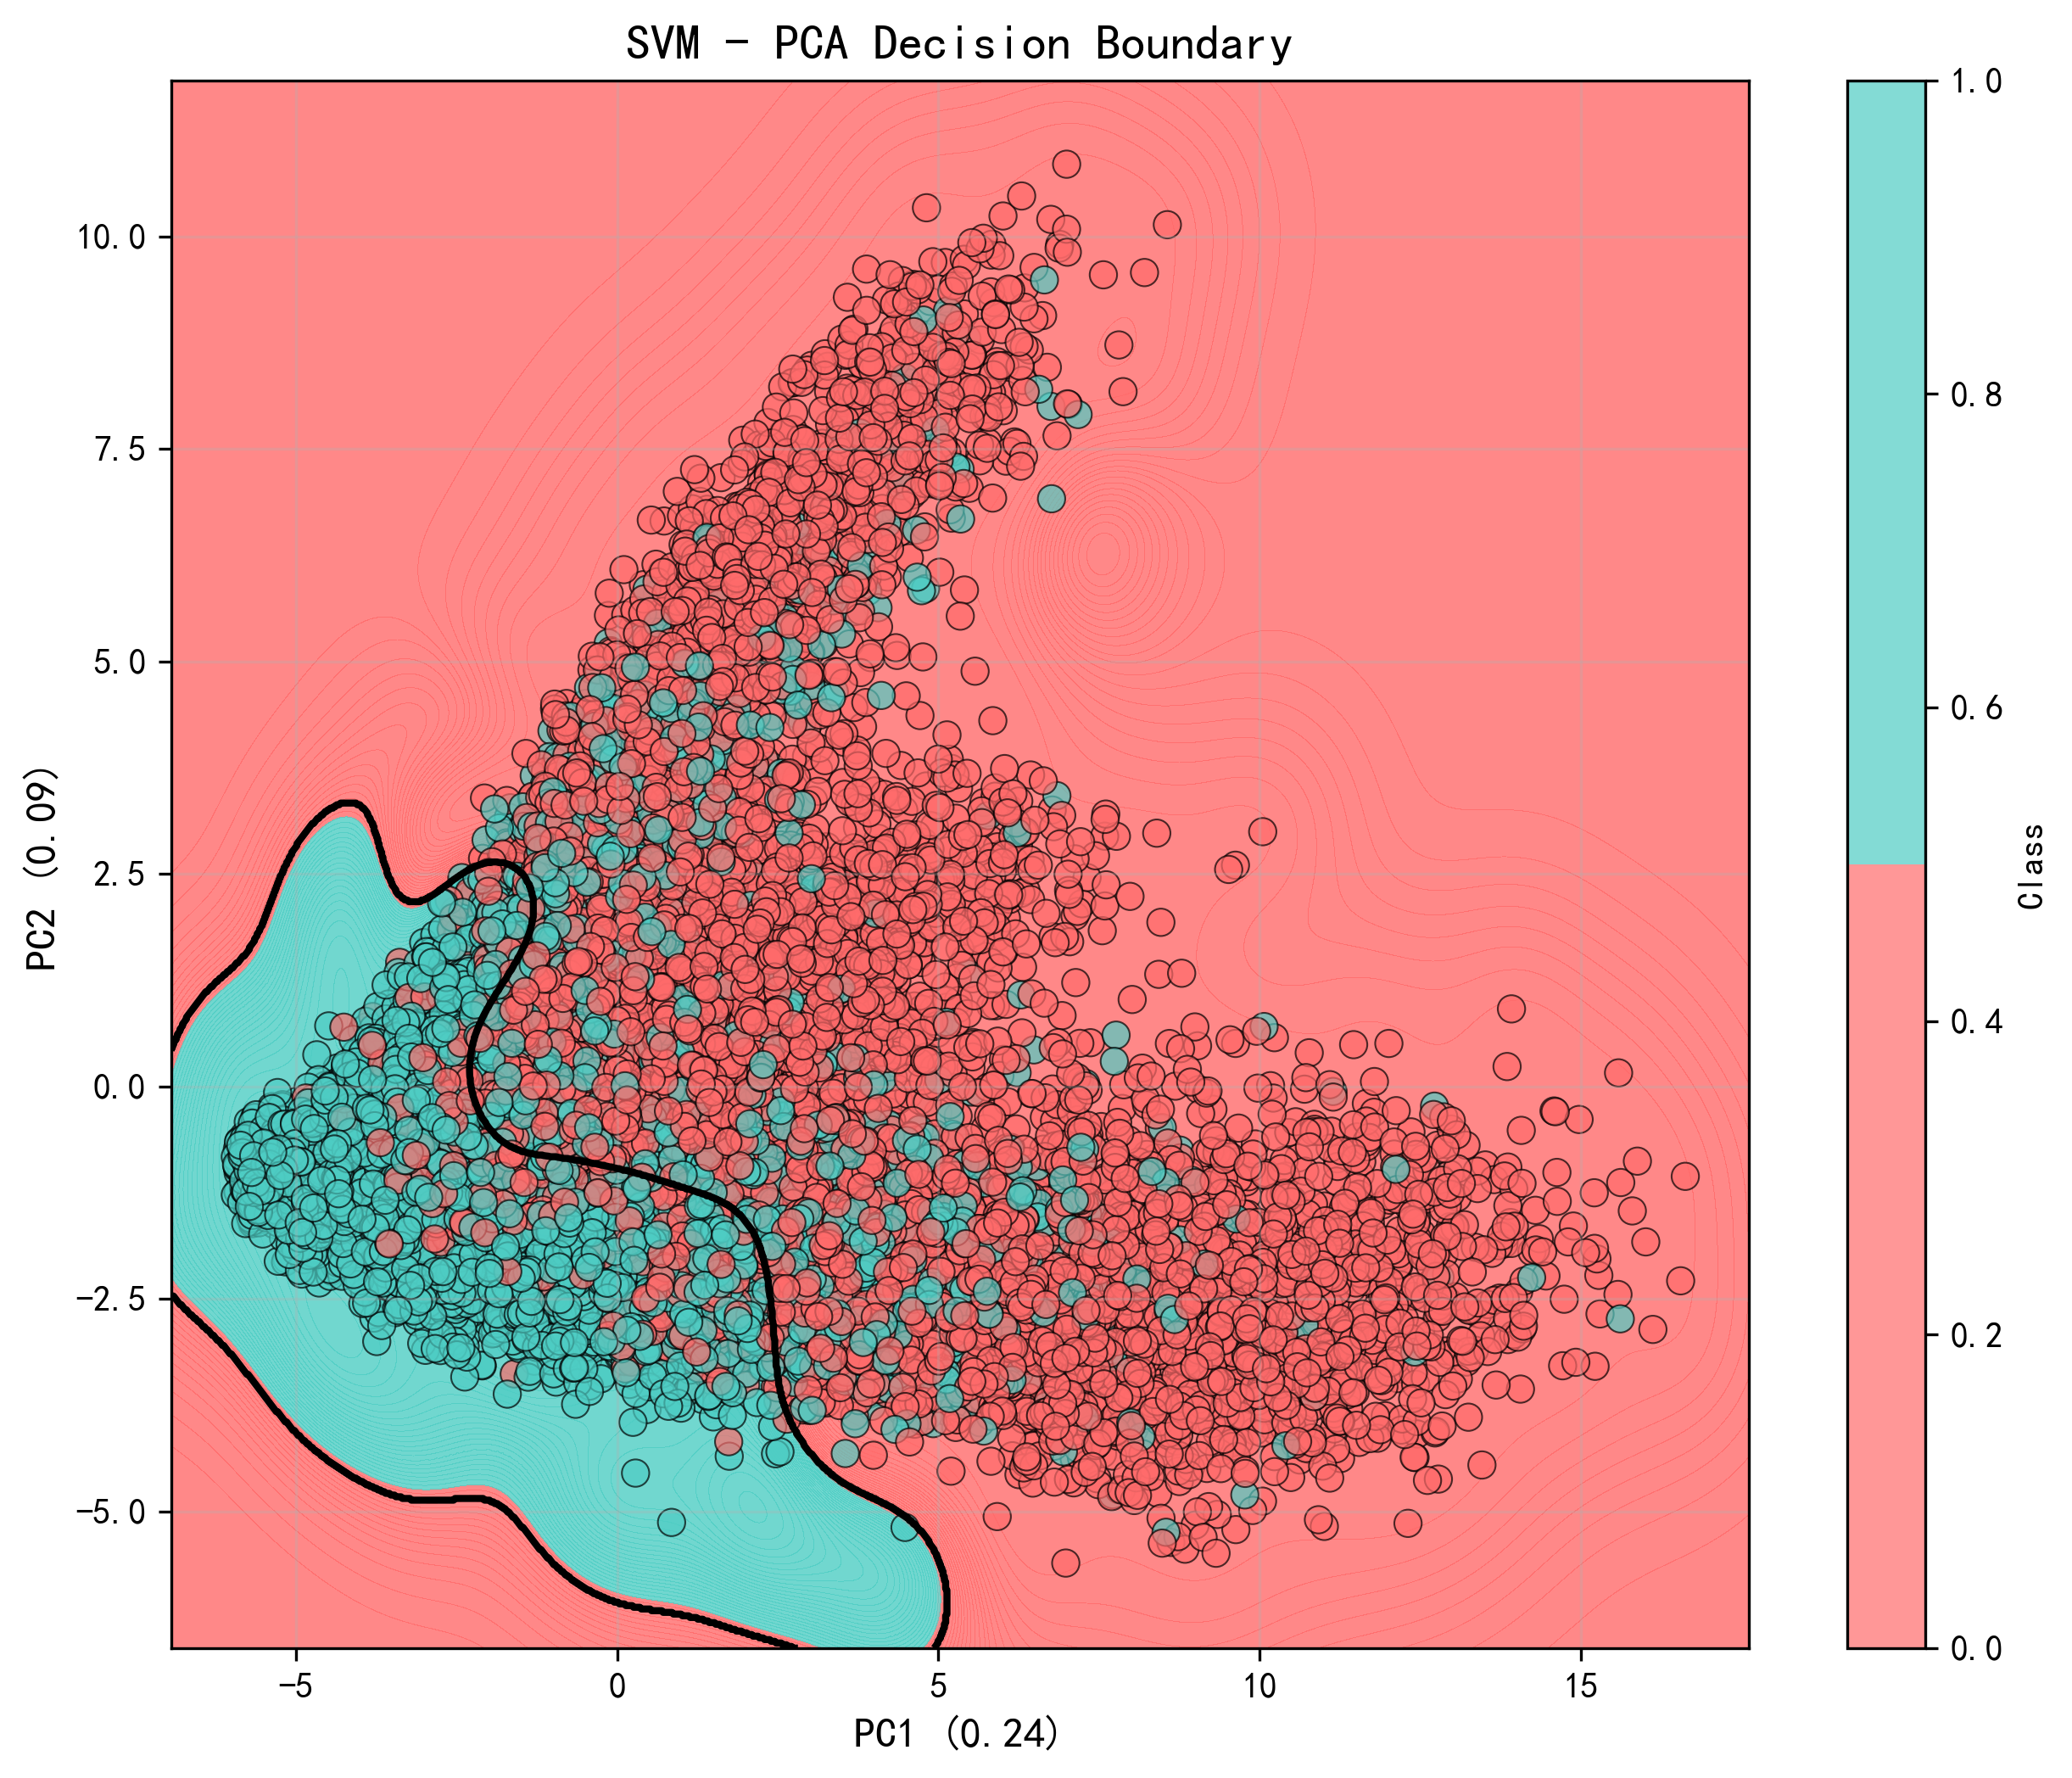
\includegraphics[width=\textwidth]{figures/svm_pca_decision_boundary.png}
        \caption{SVM决策边界}
        \label{fig:svm}
    \end{minipage}
    \hfill
    \caption{逻辑回归与SVM决策边界对比（为了方便显示，使用PCA进行降维至2维）}
    \label{fig:svmlogistic}
\end{figure}

\subsubsection{K-Means与高斯混合模型的对比分析}

无监督聚类算法旨在发现数据内在的结构与模式，而非直接预测一个已知的标签。在本研究中，我们尝试使用K-Means和高斯混合模型（GMM）对学生数据进行聚类，并使用调整兰德指数（Adjusted Rand Index, ARI）来衡量聚类结果与真实的“学业风险”标签（at\_risk）之间的一致性。实验结果显示，K-Means的ARI为0.089，而GMM的ARI仅为0.033。这一结果表明，尽管两种算法的聚类结果与真实标签的吻合度都较低，但K-Means的表现相对优于GMM。这一现象值得我们深入探讨。

从\ref{fig:kmeans}和\ref{fig:em}中我们可以直观地看到两种算法的聚类结果。K-Means倾向于生成大小相似、形状规整的球形簇，而GMM则试图拟合出更灵活的椭圆形簇。为了理解为何更灵活的GMM表现反而更差，我们需要从算法原理和数据特性两个方面进行分析。

\textbf{1. 模型假设与数据分布的匹配度差异}

两种算法的核心区别在于其根本假设。K-Means是一种基于几何距离的“硬”聚类算法，它唯一的目标是最小化簇内样本点到质心的平方和。它不对数据分布做任何概率假设，只关心几何上的远近。

相比之下，高斯混合模型（GMM）是一种基于概率模型的“软”聚类算法。其核心假设是：整个数据集是由$K$个不同的高斯（正态）分布混合生成的。它通过期望最大化（EM）算法，试图找到能最大化数据出现概率的$K$个高斯分布的参数（均值、协方差、混合系数）。这种假设赋予了GMM极大的灵活性，使其能够捕捉椭圆形、不同大小和不同方向的复杂簇结构。

然而，模型的灵活性是一把双刃剑。当模型的假设与数据的真实分布高度吻合时，它会表现出色；但当假设被违背时，其表现可能远不如更简单的模型。正如我们在EDA分析中发现的（\ref{fig:numeric_distributions}），本项目中的许多关键特征，尤其是VLE相关的点击流和活跃天数特征，都呈现出明显的右偏斜分布（right-skewed），这与GMM所依赖的正态分布假设相去甚远。K-Means不依赖于概率分布假设，因此对这种偏斜数据的容忍度更高。GMM试图用正态分布去拟合一个本质上非正态的数据群体，其结果自然是差强人意的。

\textbf{2. 模型复杂度与高维特征空间的挑战}

GMM是一个远比K-Means复杂的模型。对于一个$D$维的数据，K-Means只需要为每个簇估计$D$个参数（质心坐标）。而GMM不仅要估计均值（$D$个参数），还需要估计一个$D \times D$的协方差矩阵。在高维空间中，估计协方差矩阵需要大量的样本，否则容易产生不稳定的结果或过拟合。我们的数据集特征维度较高，GMM在拟合过程中可能受到了“维度灾难”的困扰，其复杂的参数系统反而捕捉到了数据中的噪声而非真实的结构，导致了更差的泛化表现。

反观K-Means，其简单的模型结构使其在一定程度上对维度灾难有更强的鲁棒性。它没有试图去学习数据复杂的概率结构，只是执行一个简单的几何划分任务。在这种情况下，简单即是优势。

\textbf{3. “学业风险”标签的内在可分性}

最重要的一点是，ARI值（0.089和0.033）都非常低，这强烈暗示了一个核心问题：“高风险”学生和“低风险”学生在特征空间中，本身可能就无法通过无监督聚类被清晰地分开。这两个群体之间可能没有一个天然的“鸿沟”，而是高度重叠、相互渗透的。在这种本就模糊的界限上，K-Means算法简单粗暴的“一刀切”式划分，反而可能偶然地比GMM精雕细琢的、试图寻找不存在的“优雅”概率边界的划分，产生了一个稍微好一点点的、与真实标签略有关联的结果。GMM的失败，在某种程度上，恰恰是因为它“太努力”地去寻找一个根本不存在的复杂高斯混合结构，最终找到了与真实标签几乎完全无关的聚类结果，导致其ARI值趋近于0（随机划分）。

综上所述，GMM在本任务中表现不如K-Means，并非因为模型本身优劣，而是典型的“模型与问题不匹配”的案例。数据的非正态分布特性、高维特征带来的挑战，以及“学业风险”本身可能不具备清晰聚类结构，这些因素共同导致了更简单的K-Means模型反而取得了相对更优（尽管绝对值仍然很低）的结果。这也警示我们，在选择模型时，绝非越复杂越好，深入理解数据特性和问题本质才是关键。


\begin{figure}[!htbp]
    \centering
    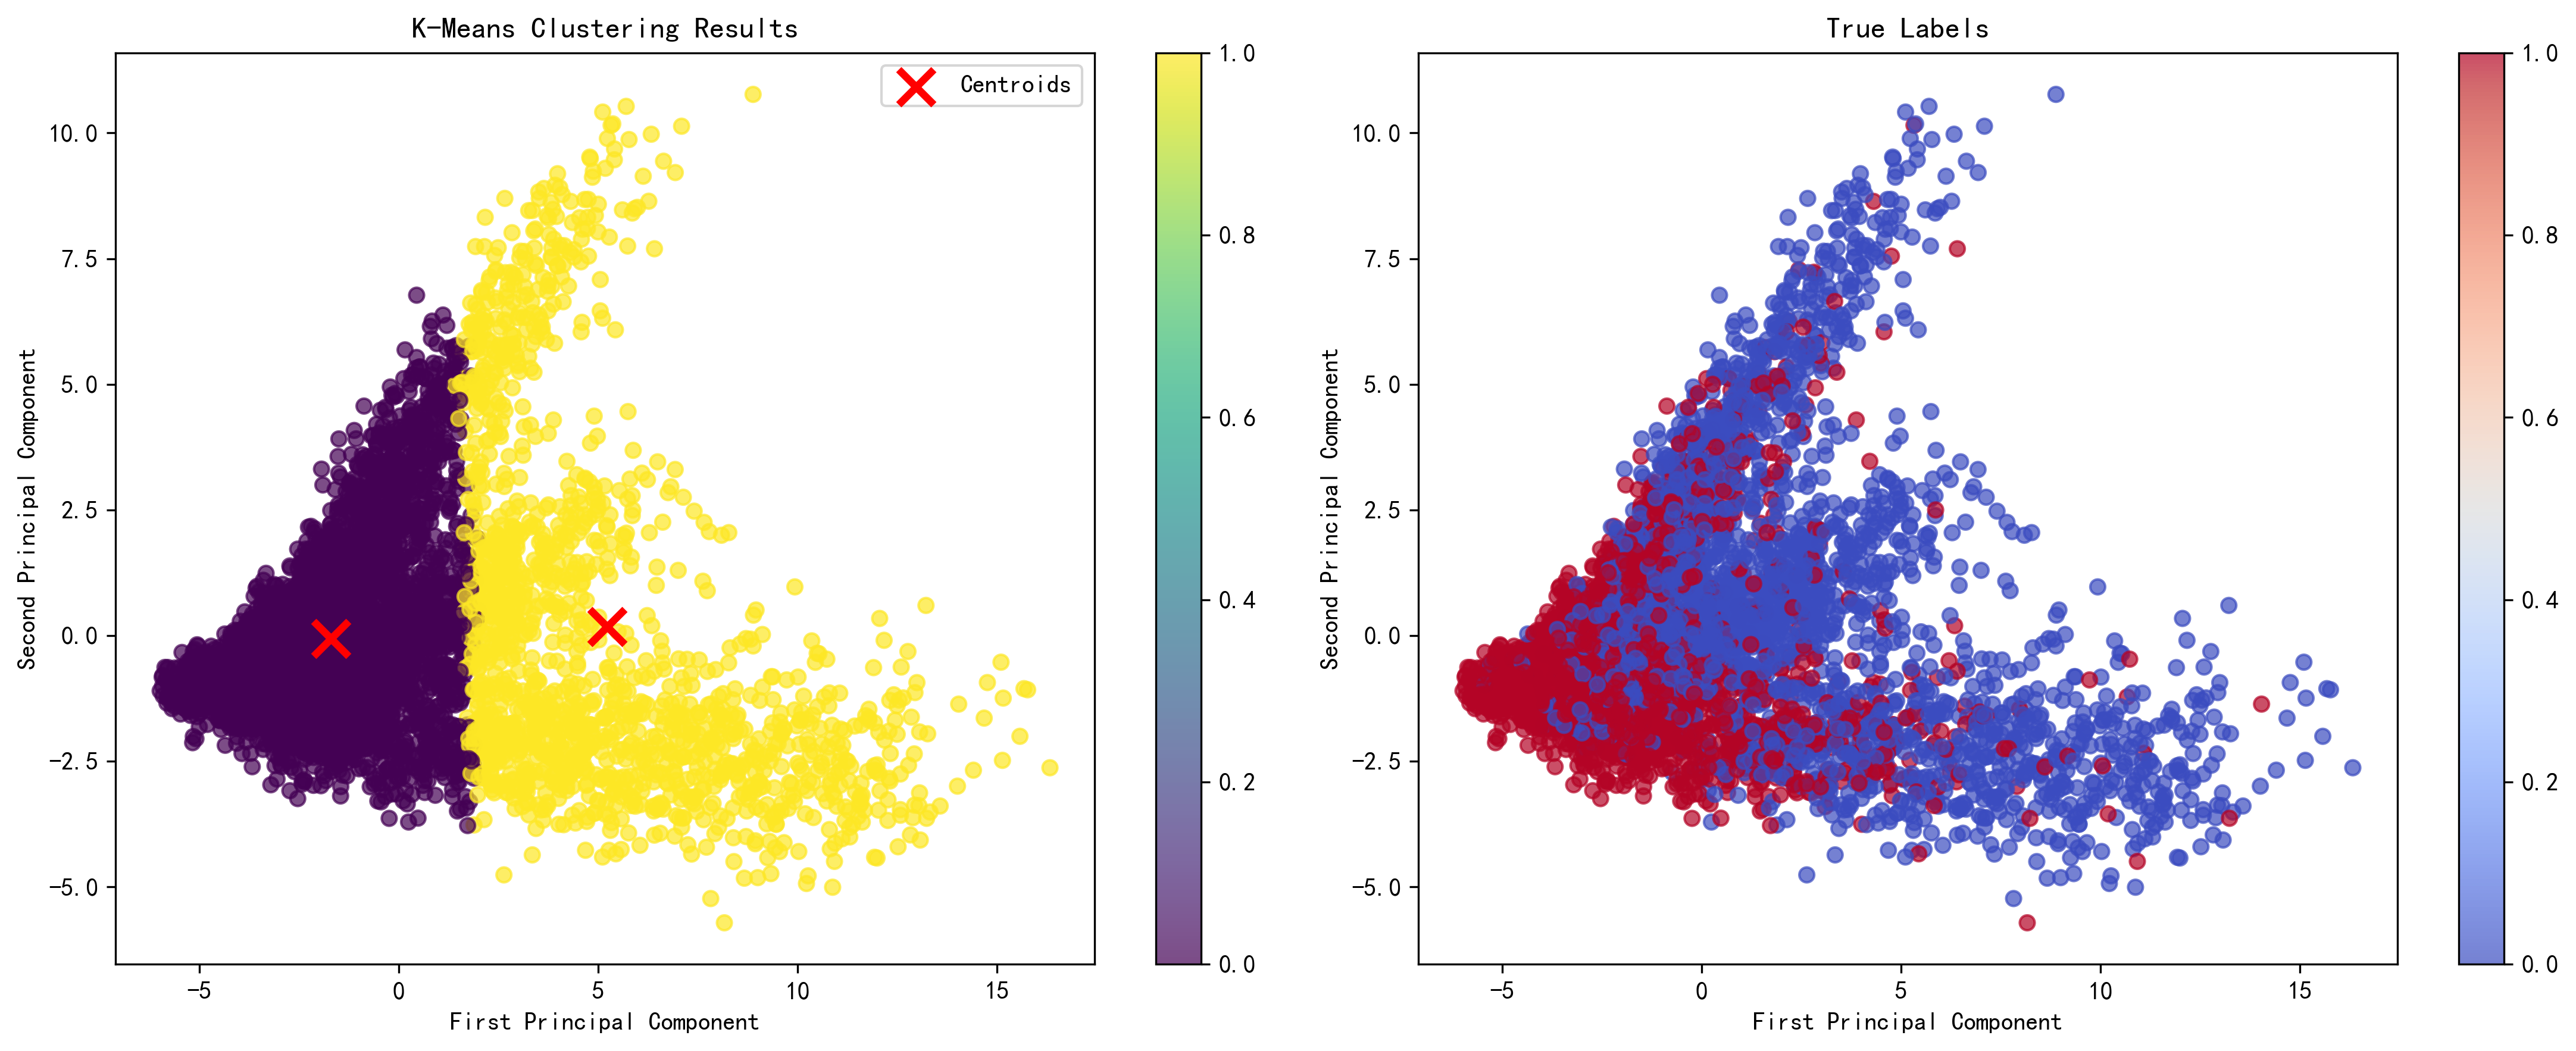
\includegraphics[width=0.5\textwidth]{figures/kmeansmodeler_clustering_results.png}
    \caption{kmeans聚类结果图}
    \label{fig:kmeans}
\end{figure}

\begin{figure}[!htbp]
    \centering
    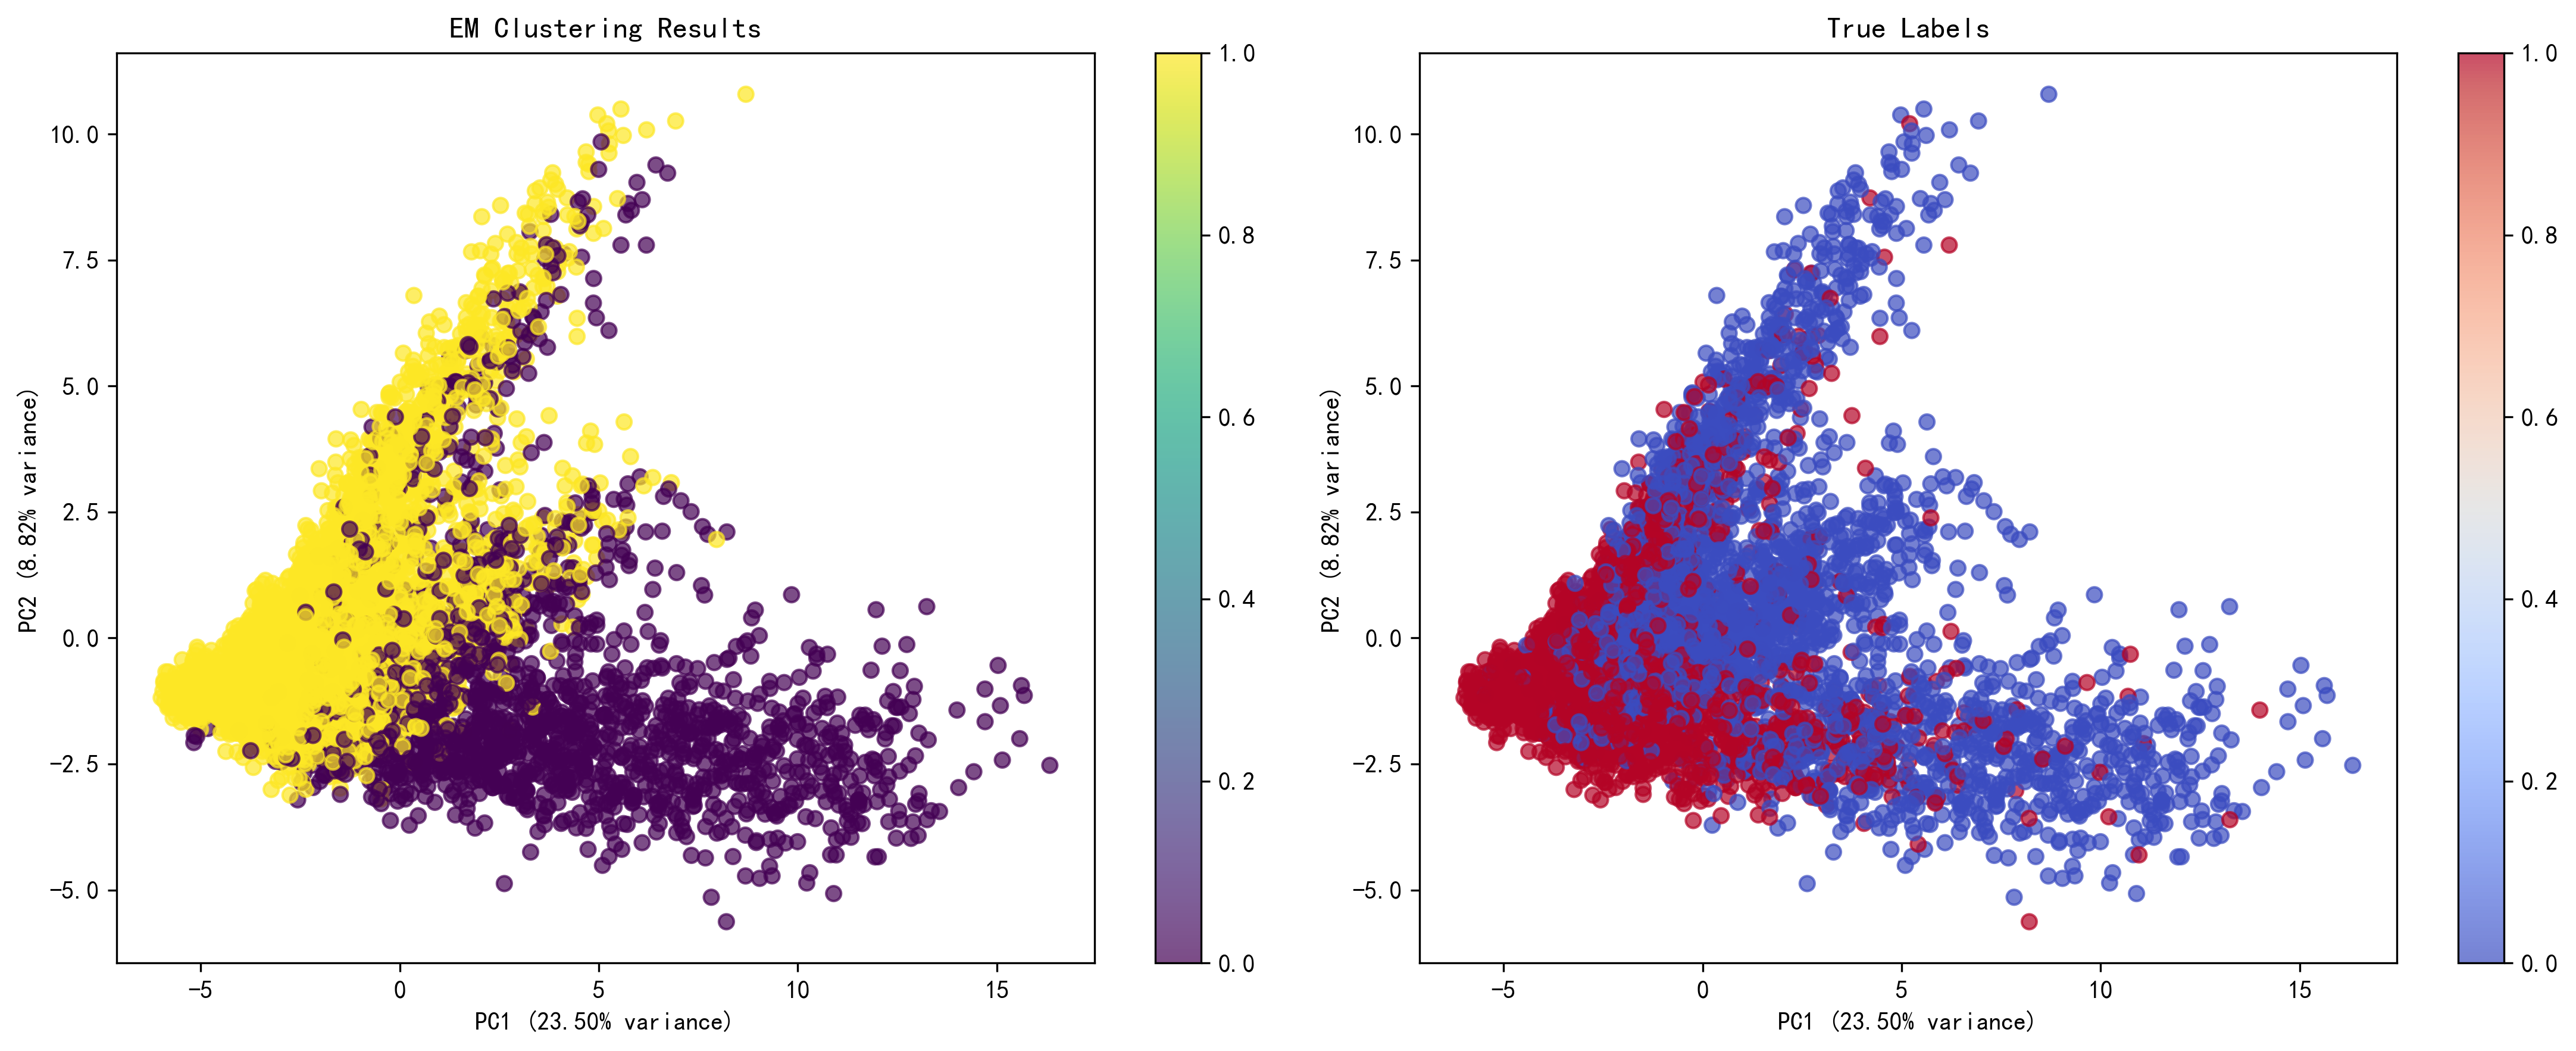
\includegraphics[width=0.5\textwidth]{figures/emmodeler_clustering_results.png}
    \caption{高斯聚类结果图}
    \label{fig:em}
\end{figure}



\subsection{模型可解释性分析 (SHAP)}
尽管复杂的机器学习模型如支持向量机（SVM）在预测准确性上表现优异，但其固有的“黑箱”特性使得我们难以理解其内部的决策逻辑。为了打开这个“黑箱”，并深入回答“哪些早期行为特征对预测风险最重要？”这一核心问题，我们引入了SHAP (SHapley Additive exPlanations)框架。SHAP基于合作博弈论中的Shapley值，能够为每一个样本的每一次预测，精确计算出每个特征的贡献度，从而提供了坚实的理论基础来解释模型的全局和局部行为。本节将对比逻辑回归和SVM的SHAP分析结果，以探究不同模型在识别关键特征上的一致性与差异性。

\subsubsection{跨模型特征重要性对比分析}
我们对逻辑回归和支持向量机（使用RBF核）这两个分别代表线性与非线性模型典范的算法进行了SHAP分析，并将它们各自的SHAP摘要图进行对比，如\ref{fig:shap_summary}所示。

\begin{figure}[!htbp]
    \centering
    \begin{minipage}[t]{0.48\textwidth}
        \centering
        
\includegraphics[width=\textwidth]{figures/logisticregressionmodeler_shap_summary.png}
        \caption{逻辑回归 SHAP 摘要图}
        \label{fig:shap_lr}
    \end{minipage}
    \hfill
    \begin{minipage}[t]{0.48\textwidth}
        \centering
        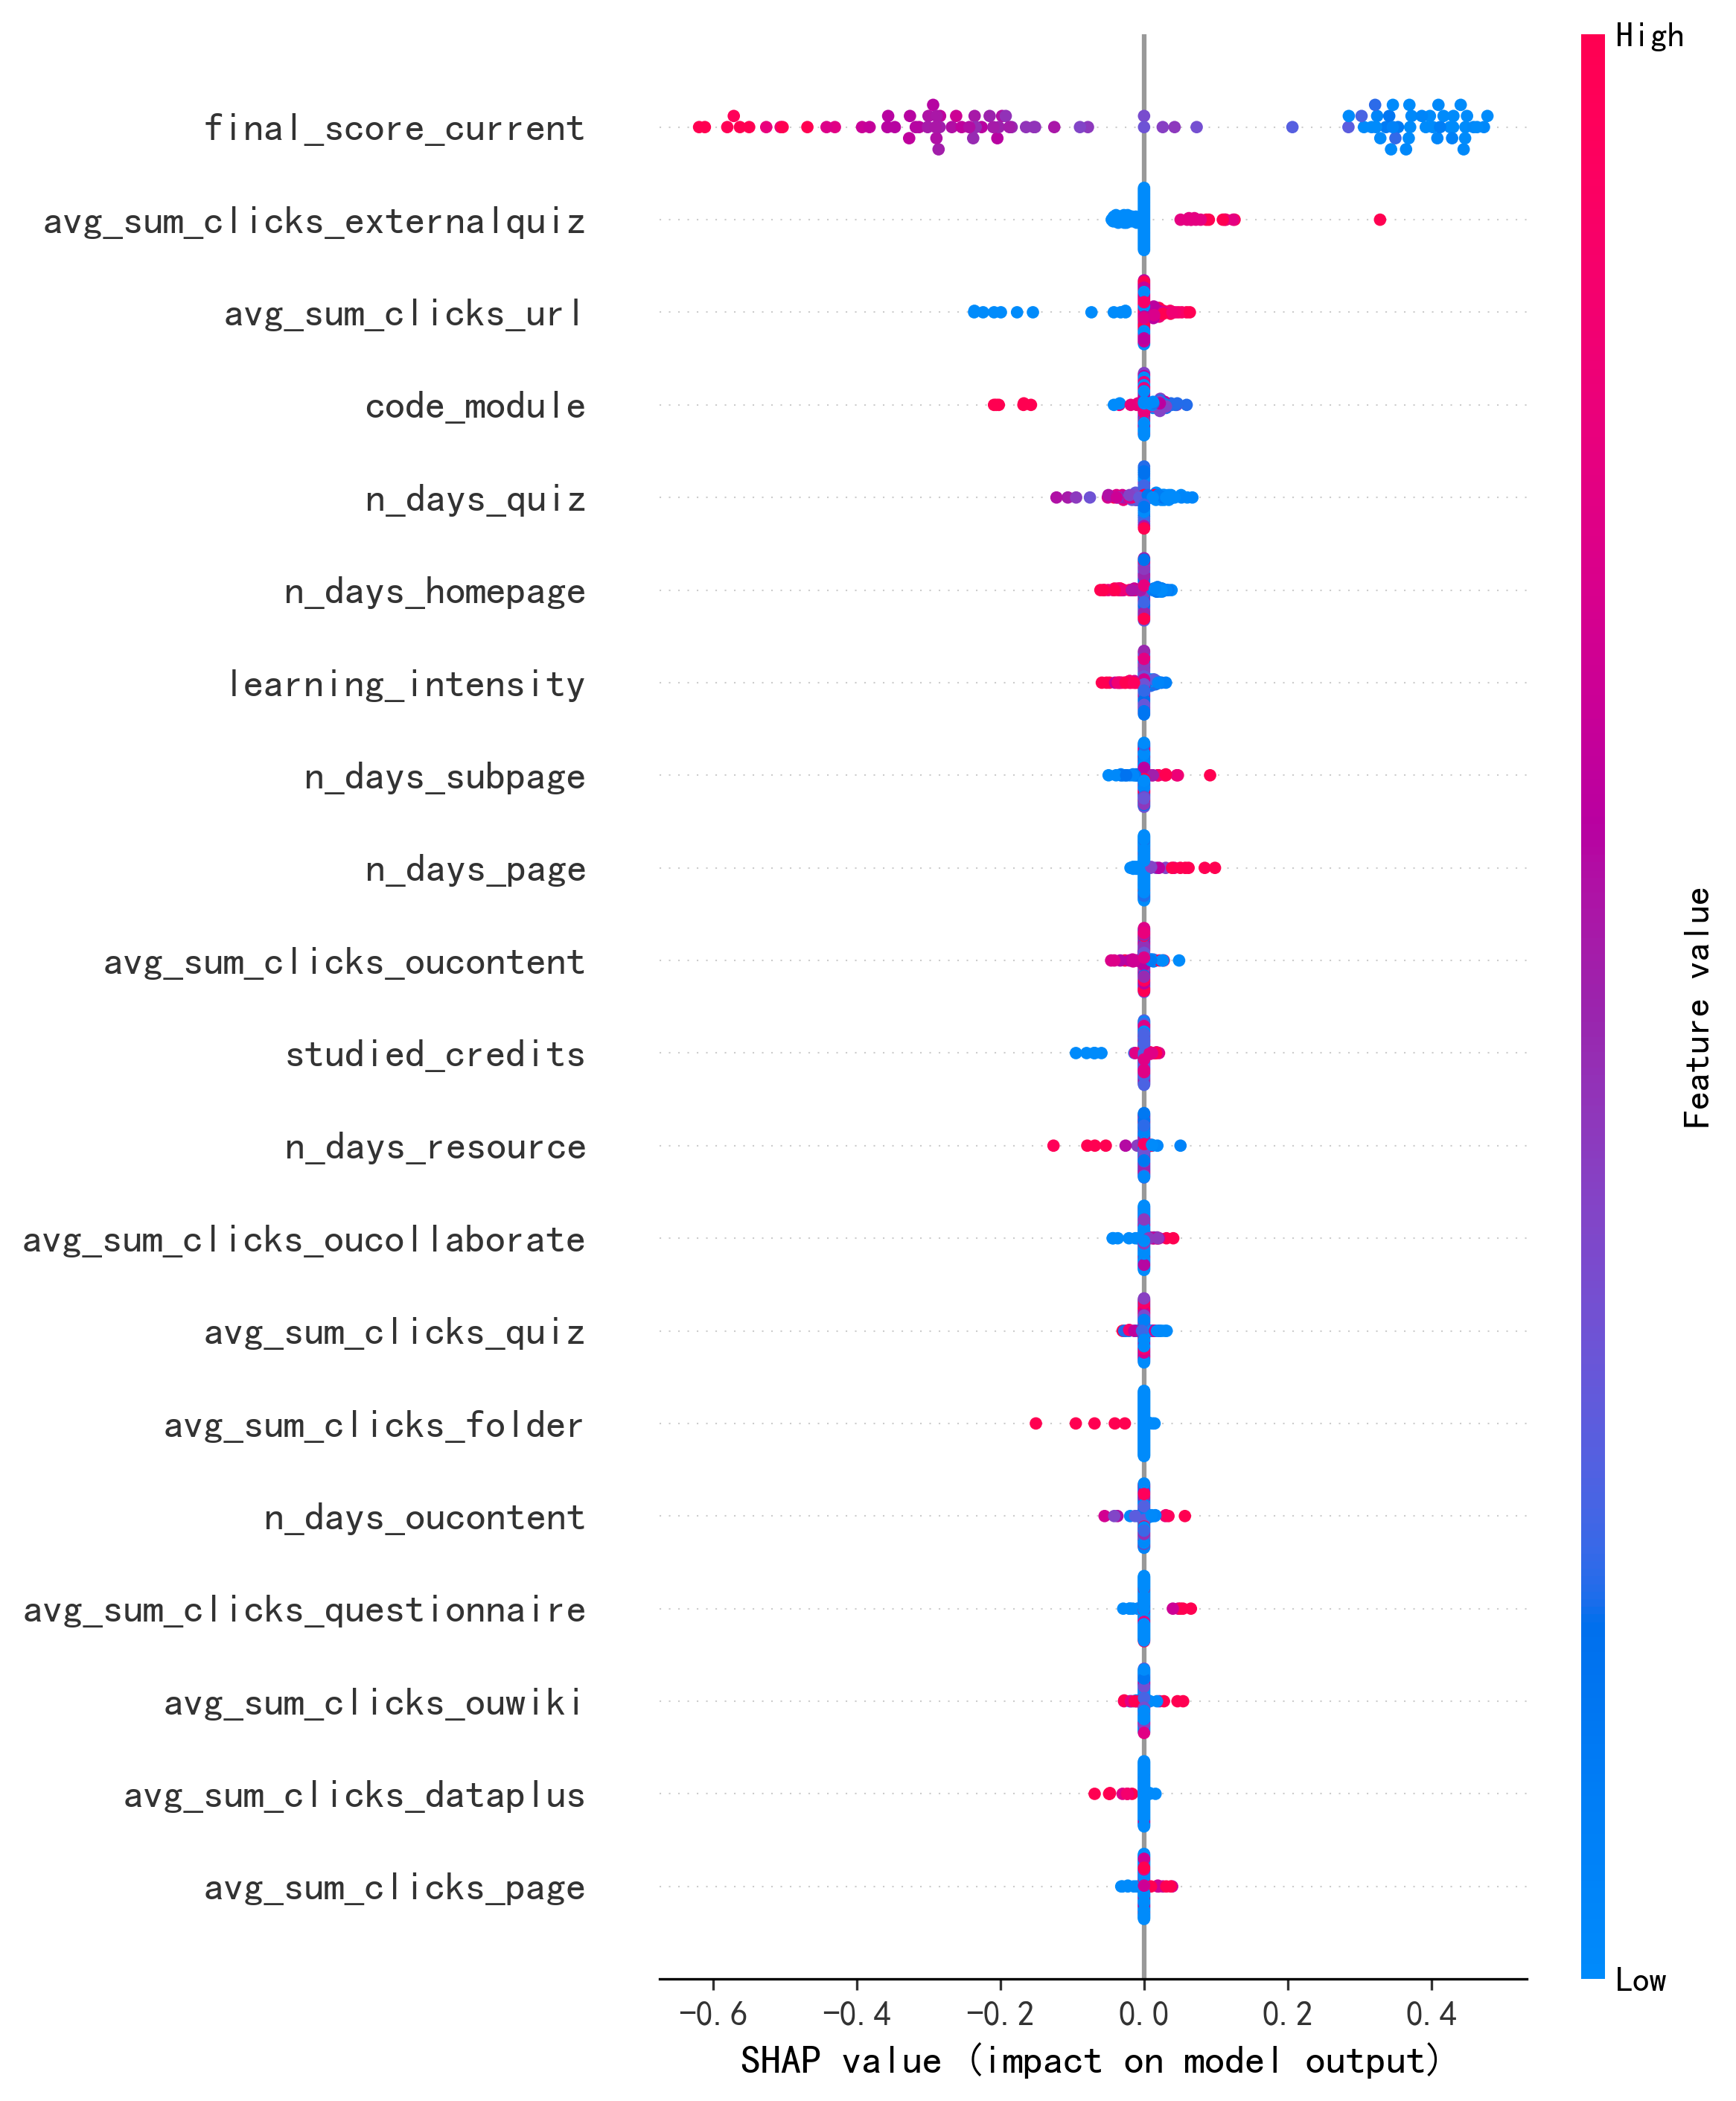
\includegraphics[width=\textwidth]{figures/svmmodeler_shap_summary.png}
        \caption{支持向量机 (SVM) SHAP 摘要图}
        \label{fig:shap_svm}
    \end{minipage}
    \caption{逻辑回归与支持向量机的SHAP摘要图对比}
    \label{fig:shap_summary}
\end{figure}

摘要图（Summary Plot）将所有测试样本的SHAP值汇总在一起，为我们揭示了全局的特征重要性。图中每一个点代表一个样本，其在X轴上的位置表示该特征对该样本预测结果的影响大小（正向或负向），颜色则表示该特征本身的数值大小（通常红色表示特征值高，蓝色表示特征值低）。通过对不同模型的摘要图进行横向比较，我们得出了以下核心发现：

\textbf{1. 高度一致的核心预测指标：}
一个极其显著的发现是，\textbf{两种机制完全不同的模型都一致地认为 \texttt{final\_score\_current}（学生当前已得评估的加权平均分）是预测学业风险的最重要特征}。从图中可以清晰地看到，该特征的SHAP值分布范围最广，对模型输出的贡献度最大。具体而言，高分值（红色点）对应负向SHAP值，有力地将预测结果推向“低风险”；而低分值（蓝色点）则对应正向SHAP值，显著增加了学生的“高风险”预测概率。这一发现跨越了线性和非线性模型的鸿沟，与我们的教育直觉完全吻合，强有力地验证了我们特征工程的有效性和模型结论的可靠性。

\textbf{2. VLE学习行为的关键作用：}
除了当前成绩，学生的学习过程性行为数据也扮演了至关重要的角色。逻辑回归和SVM均识别出了一组相似的、与VLE交互相关的关键特征，包括\texttt{n\_days\_oucontent}（访问核心课程内容天数）、\texttt{learning\_intensity}（学习强度）等。
然而，从上面也可以看出两个模型对于一些特征的关键程度衡量有一定的差异。比如gender（性别）特征在逻辑回归中被认为是一个重要的预测因子，
而在SVM中则相对不那么显著。这种差异可能源于模型对特征间交互效应的捕捉能力不同。逻辑回归作为线性模型，无法捕捉到特征间的复杂交互，
而SVM则能够通过非线性映射来学习这些关系。

\textbf{3. 模型间的细微差异：}
尽管在顶级特征上高度一致，但两个模型的SHAP图细节揭示了它们工作方式的根本不同。逻辑回归作为一个线性模型，其SHAP图中特征的影响趋势通常更清晰、单调，点的分布紧凑且呈线性。相比之下，SVM的SHAP图中点的分布更宽、更分散。这种分散性暗示了SVM正在捕捉特征间的交互效应——即一个特征的影响力可能会被另一个特征的值所调节。这是SVM作为非线性模型能力更强的体现，也是其获得更高准确率（92.25\% vs 90.39\%）的关键所在。

\subsubsection{特征依赖性深度剖析}
为了进一步探究SVM模型如何利用复杂的非线性关系，我们使用SHAP依赖图（Dependence Plot）对最重要的特征 \texttt{final\_score\_current} 进行深度剖析，以揭示其对模型预测结果的具体影响模式。

\begin{figure}[!htbp]
    \centering
    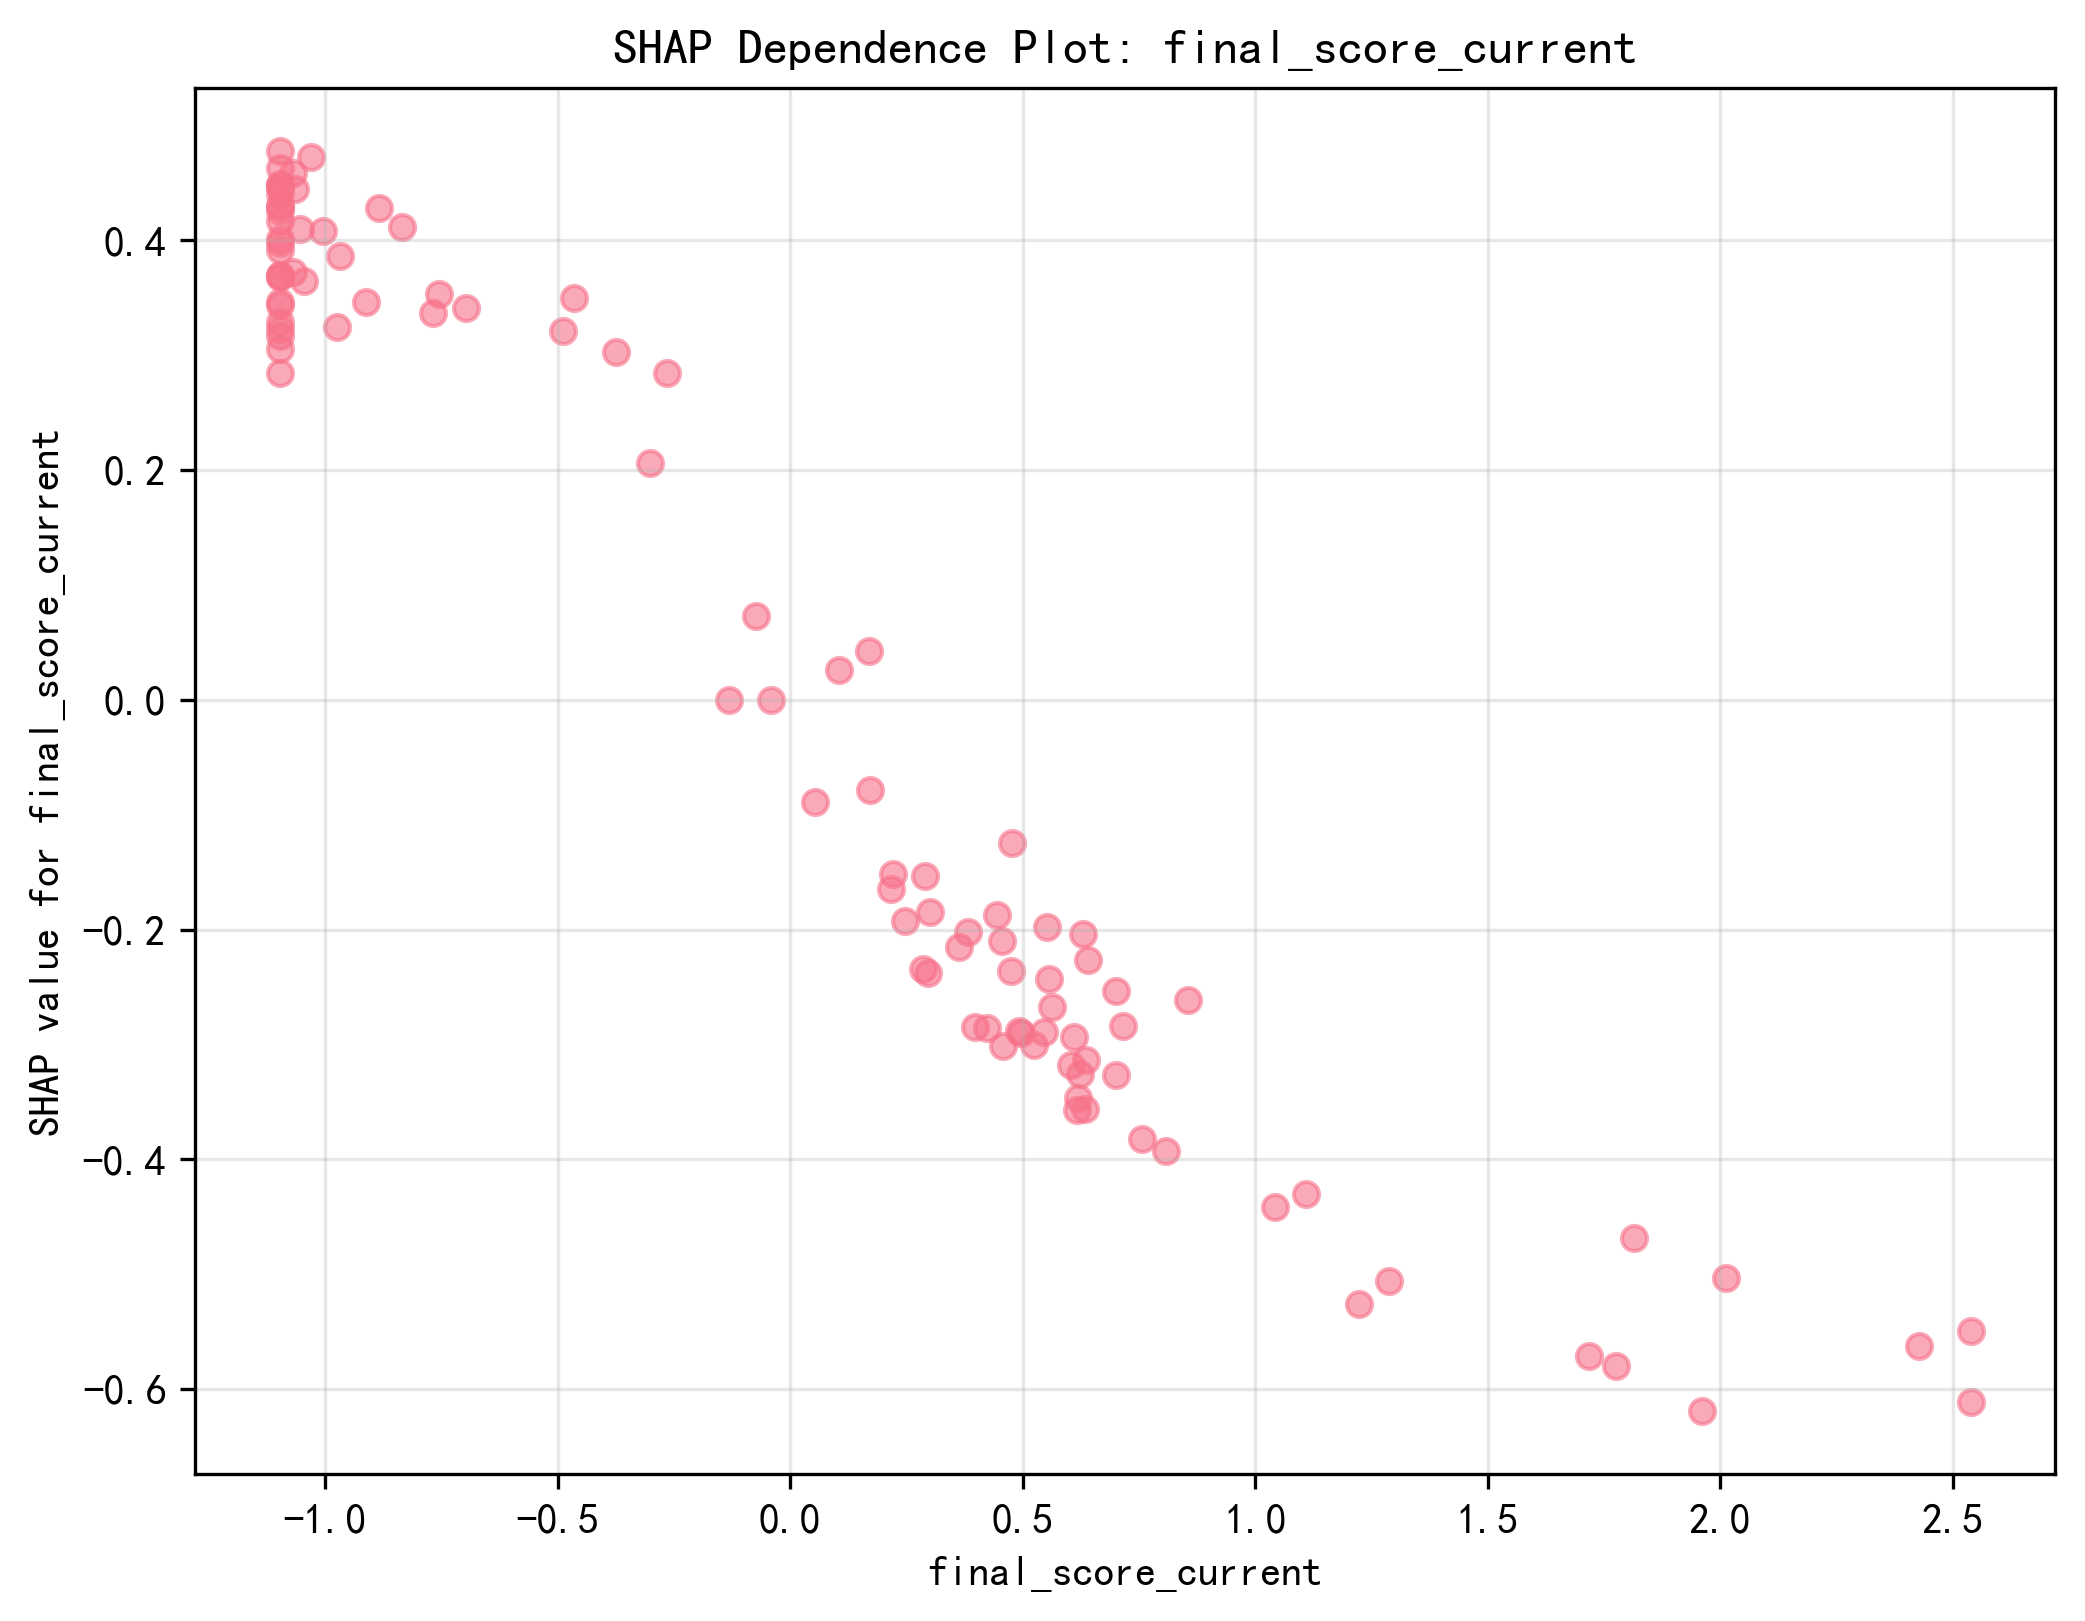
\includegraphics[width=0.6\textwidth]{figures/svmmodeler_shap_dependence_final_score_current.png}
    \caption{支持向量机模型 \texttt{final\_score\_current} 特征SHAP依赖图}
    \label{fig:shap_dependence_svm}
\end{figure}

如\autoref{fig:shap_dependence_svm}所示，该图清晰地展示了学生当前得分 (\texttt{final\_score\_current}) 和其对应的SHAP值之间的关系。我们可以观察到几个关键趋势：
\begin{itemize}
    \item \textbf{明确的负相关性：} 整体上，特征的SHAP值随着分数的增高而降低。高分值（X轴右侧）对应着负的SHAP值，这意味着高分会强烈地将模型的预测推向“低风险”类别。相反，低分值（X轴左侧）则对应着正的SHAP值，显著增加了学生被判定为“高风险”的概率。
    \item \textbf{显著的非线性效应：} 这种关系并非一条直线。在分数较低的区间，SHAP值处于一个较高的正值平台，说明一旦分数低于某个阈值，其带来的风险效应非常显著。而随着分数提高，SHAP值下降的速度先是加快，之后在分数较高的区域逐渐变得平缓。这种“S”形或“ hockey-stick”形的曲线揭示了模型捕捉到的非线性关系：成绩对风险的影响并非是等比例的，在及格线附近的变化尤为关键。
\end{itemize}
这个发现非常有价值，它表明SVM模型不仅仅是简单地认为“分数越高，风险越低”，而是学习到了一个更细致的、非线性的影响模式。这种能力也是SVM这类模型相比逻辑回归等线性模型在处理复杂问题时的核心优势之一。

综上所述，SHAP分析不仅极大地增强了我们对SVM这类复杂模型决策过程的信任度，更重要的是，它为我们提供了一致且可操作的洞见。不同模型交叉验证的核心发现——即\textbf{学生的即时学业表现 (\texttt{final\_score\_current}) 和学习过程的参与度 (VLE活动特征) 是预测未来学业风险的最关键因素}——为教育者实施早期、精准的干预提供了强有力的数据支持。

\subsection{超参数优化分析}
机器学习模型的性能在很大程度上取决于其超参数的选择。传统的网格搜索（Grid Search）方法虽然详尽，但在高维参数空间中会遭遇“维度灾难”，计算成本呈指数级增长。随机搜索（Random Search）虽然更高效，但缺乏方向性。为了系统性且高效地发掘每个模型的最佳性能，本项目引入了业界领先的自动化超参数优化框架Optuna。Optuna采用基于树状结构Parzen估计器（Tree-structured Parzen Estimator, TPE）的贝叶斯优化算法，能够智能地利用历史试验的结果来指导未来的搜索方向，将更多的计算资源投入到更有希望的参数区域，同时，其激进的剪枝（Pruning）策略可以及早终止没有潜力的试验，从而在有限的时间内找到更优的解。本节将以逻辑回归和随机森林为例，深入分析Optuna的优化过程。

我们利用Optuna的可视化功能，对优化过程进行了深入分析。以逻辑回归为例(\ref{fig:optuna_lr})，其核心超参数是正则化强度\texttt{C}。参数重要性图显示，\texttt{C}值是影响模型性能的决定性因素。优化历史图则记录了20次迭代过程中目标函数值（F1-Score）的变化，可以看到F1分数稳步提升并最终收敛在0.90附近，表明Optuna成功地为模型找到了一个表现优异的参数配置。

\begin{figure}[!htbp]
    \centering
    \begin{minipage}[t]{0.48\textwidth}
        \centering
        
\includegraphics[width=\textwidth]{figures/logisticregressionmodeler_optuna_history.png}
        \caption{逻辑回归优化历史图}
        \label{fig:optuna_lr_history}
    \end{minipage}
    \hfill
    \begin{minipage}[t]{0.48\textwidth}
        \centering
        
\includegraphics[width=\textwidth]{figures/logisticregressionmodeler_optuna_param_importance.png}
        \caption{逻辑回归参数重要性图}
        \label{fig:optuna_lr_imp}
    \end{minipage}
    \caption{逻辑回归Optuna优化过程可视化}
    \label{fig:optuna_lr}
\end{figure}

对于结构更复杂的随机森林模型，其超参数空间更为庞大（如\texttt{n\_estimators}, \texttt{max\_depth}, \texttt{min\_samples\_leaf}等）。Optuna的优势在此刻体现得淋漓尽致。通过平行坐标图（Parallel Coordinate Plot, \ref{fig:optuna_rf_parallel}），我们可以直观地观察到不同超参数组合与最终模型性能的关系。图中的每一条线代表一次试验，线条的颜色代表了目标函数值（本例中，蓝色表示更好的F1分数）。我们可以清晰地看到，表现最好的蓝色线条普遍集中在\texttt{max\_depth}较大、\texttt{min\_samples\_leaf}较小、\texttt{n\_estimators}较高的区域，这为我们理解模型偏好提供了宝贵的洞见。而切片图（Slice Plot, \ref{fig:optuna_rf_slice}）则进一步展示了单个超参数对性能的影响曲线，帮助我们确认最佳参数的取值范围。

\begin{figure}[!htbp]
    \centering
    \begin{minipage}[t]{0.48\textwidth}
        \centering
        
\includegraphics[width=\textwidth]{figures/randomforestmodeler_optuna_parallel_coordinate.png}
        \caption{随机森林平行坐标图}
        \label{fig:optuna_rf_parallel}
    \end{minipage}
    \hfill
    \begin{minipage}[t]{0.48\textwidth}
        \centering
        
\includegraphics[width=\textwidth]{figures/randomforestmodeler_optuna_slice.png}
        \caption{随机森林切片图}
        \label{fig:optuna_rf_slice}
    \end{minipage}
    \caption{随机森林Optuna优化过程可视化}
    \label{fig:optuna_rf}
\end{figure}

综上所述，引入Optuna不仅是一个提升模型分数的工程步骤，更是一个深入的分析过程。它不仅将我们从繁琐的手动调参中解放出来，其丰富的可视化工具更赋予了我们洞察“黑箱”模型行为的能力，加深了我们对超参数如何影响模型学习过程的理解。


\section{总结与展望}
\subsection{工作总结}
本项目成功设计并实现了一个基于OULAD数据集的、端到端的学业风险预警系统。我们构建了一个模块化、自动化的机器学习流水线，并系统性地实现、优化和评估了六种覆盖不同范式的机器学习模型。通过对实验结果进行多维度的对比分析，我们得出以下核心结论：

\begin{enumerate}
    \item \textbf{非线性关系是关键：} 在准确性方面，能够捕捉非线性关系的复杂模型，如支持向量机（准确率92.25\%）和随机森林（92.15\%），其性能显著优于线性模型逻辑回归（90.39\%）。这有力地证明了学业风险的预测问题本质上是高度非线性的，学生的学习行为特征与最终成果之间存在复杂的交互作用。

    \item \textbf{性能与效率的权衡是核心考量：} 实验结果清晰地揭示了模型性能与计算效率之间的巨大权衡。支持向量机虽然准确率最高，但其训练时间长达约46分钟，计算成本极为高昂。而逻辑回归和决策树虽然性能稍逊，但训练速度极快（均在20秒以内），展现了在需要快速迭代或大规模部署场景下的巨大优势。

    \item \textbf{模型可解释性的价值得以验证：} 通过引入SHAP框架，我们成功打开了SVM和随机森林等“黑箱”模型。分析发现，尽管模型机制迥异，但逻辑回归和SVM均一致地识别出 \texttt{final\_score\_current}（学生当前得分）是决定学业风险的最关键特征。此外，\texttt{n\_days\_oucontent}（访问课程内容天数）等一系列VLE交互特征也显示出高度的重要性。这些发现不仅验证了我们特征工程的有效性，更重要的是为教育干预提供了明确、可操作的切入点。

    \item \textbf{无监督方法的局限性：} K-Means和高斯混合模型的聚类结果与真实的风险标签吻合度很低（ARI分别为0.089和0.033）。这表明，在当前的特征空间中，“高风险”与“低风险”学生群体并非自然分离的、界限清晰的簇，而是高度重叠、相互渗透的。这警示我们，不能想当然地认为不同标签的群体在无监督视角下也具有天然的可分性。
\end{enumerate}

综上所述，本项目不仅交付了一个功能完整的预测系统，更重要的是，通过严谨的对比实验和深度分析，为如何在具体的学业风险预警场景中选择合适的模型、平衡不同维度（准确性、效率、可解释性）的需求，提供了宝贵的数据支持和实践洞见。

\subsection{未来展望}
本研究为学业风险预警提供了一个坚实的基础，但仍有许多可以探索和改进的方向，我们对未来的工作提出以下展望：

\begin{enumerate}
    \item \textbf{深化特征工程：} 目前的特征主要基于聚合统计量。未来的工作可以引入更复杂的时序特征工程，例如分析学生在VLE活动上的时间序列模式（如学习行为的周期性、活跃度的变化趋势等），或使用深度学习模型（如LSTM）直接从原始点击流序列中提取特征，这可能捕捉到更多与风险相关的动态行为模式。

    \item \textbf{探索更前沿的模型：} 本项目主要关注经典模型，未来可以引入当前在工业界和竞赛中表现更为出色的梯度提升树模型，如XGBoost、LightGBM和CatBoost。这些模型通常能在表格数据上达到顶尖的性能，并且内置了高效的特征重要性评估和缺失值处理机制。

    \item \textbf{拓展问题定义与任务：} 目前的任务是二元分类。未来可以将其拓展为更精细化的多分类任务（例如，预测“低风险”、“中度风险”、“高度风险”、“退课”等），甚至可以构建一个多标签模型，同时预测风险等级和可能导致风险的主要原因（如“参与度不足”、“评估困难”等），为教师提供更具针对性的干预建议。
\end{enumerate}


% =============================================
% Part 5： 参考文献
% =============================================
%在reference.bib文件中填写参考文献，此处自动生成

\newpage
\bibliographystyle{ieeetr}
\bibliography{reference}

\end{document}